%%%%%%%%%%%%%%%%%%%%%%%%%%%%%%%%%%%%%%%%%%%%%%%%%%%%%%%%%%%%%%%%%%%%
%% Automobile Membrane Computing: A Biological Semiconductor
%% Surface Architecture for Autonomous Navigation via Categorical
%% Trajectory Completion in Bounded Phase Space
%%
%% Author: Kundai Farai Sachikonye
%% Technical University of Munich
%%%%%%%%%%%%%%%%%%%%%%%%%%%%%%%%%%%%%%%%%%%%%%%%%%%%%%%%%%%%%%%%%%%%
\documentclass[twocolumn,10pt]{article}
\usepackage[utf8]{inputenc}
\usepackage[T1]{fontenc}
%%% Packages
\usepackage[margin=1in]{geometry}
\usepackage{amsmath,amssymb,amsthm}
\usepackage{graphicx}
\usepackage[colorlinks=true,linkcolor=blue,citecolor=blue,urlcolor=blue]{hyperref}
\usepackage{booktabs}
\usepackage{siunitx}
\usepackage{algorithm}
\usepackage{algorithmic}
\usepackage{physics}
\usepackage{float}
\usepackage{caption}
\usepackage{subcaption}
\usepackage{enumitem}
\usepackage{mathtools}
\usepackage{tabularx}
\usepackage{longtable}

%%% Theorem environments
\newtheorem{theorem}{Theorem}[section]
\newtheorem{lemma}[theorem]{Lemma}
\newtheorem{proposition}[theorem]{Proposition}
\newtheorem{corollary}[theorem]{Corollary}
\newtheorem{conjecture}[theorem]{Conjecture}
\theoremstyle{definition}
\newtheorem{definition}[theorem]{Definition}
\newtheorem{axiom}{Axiom}
\newtheorem{example}[theorem]{Example}
\theoremstyle{remark}
\newtheorem{remark}[theorem]{Remark}

%%% Custom commands
\newcommand{\Sent}{S_{\mathrm{ent}}}
\newcommand{\Sk}{S_k}
\newcommand{\St}{S_t}
\newcommand{\Se}{S_e}
\newcommand{\Sosc}{S_{\mathrm{osc}}}
\newcommand{\Scat}{S_{\mathrm{cat}}}
\newcommand{\Spart}{S_{\mathrm{part}}}
\newcommand{\kB}{k_{\mathrm{B}}}
\newcommand{\Ocat}{\hat{O}_{\mathrm{cat}}}
\newcommand{\Ophys}{\hat{O}_{\mathrm{phys}}}
\newcommand{\dcat}{d_{\mathrm{cat}}}
\newcommand{\beff}{b_{\mathrm{eff}}}
\newcommand{\tauopt}{\tau_{\mathrm{opt}}}
\newcommand{\xicoh}{\xi_{\mathrm{coh}}}
\newcommand{\Nens}{N_{\mathrm{ens}}}
\newcommand{\Rcompute}{R_{\mathrm{compute}}}
\newcommand{\VGamma}{V_{\Gamma}}

\title{\textbf{Automobile Membrane Computing: A Biological Semiconductor Surface Architecture for Autonomous Navigation via Categorical Trajectory Completion in Bounded Phase Space}}

\author{
Kundai Farai Sachikonye\\
AIMe Registry for Artificial Intelligence\\
\texttt{kundai.sachikonye@bitspark.com}
}

\date{March 2026}

\begin{document}

\maketitle

\begin{abstract}
We present a fundamentally new architecture for autonomous vehicle navigation in which the entire vehicle surface is wrapped in a biological lipid membrane that simultaneously serves as sensor, computer, and actuator interface. This architecture rests on the triple equivalence $\Sosc = \Scat = \Spart = \kB M \ln n$ established in prior work, which demonstrates that observation, computation, and processing are identical operations---categorical address resolution in $S$-entropy space. The membrane, derived from bounded phase space with zero free parameters (bilayer thickness \SI{4.0}{nm}, area per lipid \SI{0.64}{nm^2}, bending modulus $19\,\kB T$), provides $\sim 10^{28}$ operations per second over a typical vehicle surface area of \SI{10}{m^2}. Environmental information is encoded in phase-locked $\mathrm{O}_2$ ensembles ($\sim 10^4$ molecules per ensemble, coherence length $\xicoh \approx \SI{14}{nm}$) that transitively couple the membrane to every atmospheric perturbation---including other vehicles, obstacles, road surfaces, and weather---through the chain membrane $\leftrightarrow$ $\mathrm{O}_2$ $\leftrightarrow$ environment. Navigation is achieved via backward trajectory completion at $O(\log_3 N)$ complexity rather than forward simulation at $O(N)$, eliminating chaotic prediction failure. Sufficiency recognition---a convergence test on phase-lock quality---replaces probabilistic prediction entirely, guaranteeing that the vehicle stops whenever information is insufficient. The categorical distance metric satisfies $\partial \dcat / \partial \tau_{\mathrm{optical}} = 0$, rendering the system immune to occlusion, fog, darkness, and all photon-propagation-dependent failure modes. We prove that this architecture solves every major failure mode of conventional autonomous vehicles---limited sensor range, occlusion, GPS dependency, prediction failure, computational cost, weather sensitivity, and edge-case vulnerability---through a single biological surface that replaces LiDAR, radar, cameras, GPS, and IMU with a membrane costing orders of magnitude less and consuming milliwatts rather than kilowatts.
\end{abstract}

%%%%%%%%%%%%%%%%%%%%%%%%%%%%%%%%%%%%%%%%%%%%%%%%%%%%%%%%%%%%%
\part{Foundations}
\label{part:foundations}
%%%%%%%%%%%%%%%%%%%%%%%%%%%%%%%%%%%%%%%%%%%%%%%%%%%%%%%%%%%%%

%%%%%%%%%%%%%%%%%%%%%%%%%%%%%%%%%%%%
\section{Introduction}
\label{sec:introduction}
%%%%%%%%%%%%%%%%%%%%%%%%%%%%%%%%%%%%

\subsection{The Autonomous Driving Problem}

The autonomous vehicle (AV) industry has invested over \$100 billion in the past decade pursuing a paradigm that is fundamentally flawed \cite{thrun2006stanley, schwarting2018planning, bojarski2016end}. The conventional approach decomposes autonomous driving into a pipeline: \emph{sense} the environment using LiDAR, cameras, radar, and GPS; \emph{fuse} these disparate sensor modalities into a coherent world model; \emph{predict} the future trajectories of all agents; \emph{plan} an optimal path; and \emph{control} the vehicle along that path. Each stage introduces errors, and the pipeline's serial structure means errors compound catastrophically.

LiDAR provides precise range measurements but fails in heavy rain, fog, and dust \cite{kaplan2017understanding}. Cameras offer rich semantic information but are blind at night and in adverse weather. Radar penetrates weather but provides poor angular resolution. GPS requires satellite visibility and achieves only meter-level accuracy in urban canyons \cite{kaplan2017understanding}. The fusion of these modalities requires Kalman filtering or deep neural networks that are brittle, opaque, and provably unable to handle the combinatorial explosion of edge cases encountered in real driving \cite{schwarting2018planning}.

The prediction problem is worse. Forward simulation of multi-agent trajectories is chaotic in the Lyapunov sense: small perturbations in initial conditions produce exponentially divergent predictions \cite{helbing2001traffic}. No amount of computational power can overcome this fundamental limitation. The industry's response---collecting ever more training data for ever larger neural networks---is a brute-force assault on a problem that admits no brute-force solution.

The planning problem inherits all upstream errors. A* and RRT-based planners operate at $O(N)$ complexity in the number of environment states $N$, which for a realistic urban environment with $10^6$ discrete states and $10^2$ agents yields planning horizons of seconds at best \cite{urmson2008autonomous}. Real-time replanning at \SI{10}{Hz} with $10^3$~ms latency leaves no margin for the unexpected.

The control problem---converting planned trajectories into actuator commands---is perhaps the only well-solved component, yet it inherits the accumulated errors of every upstream stage. The result is a system that works well in controlled environments (highways, clear weather, light traffic) and fails unpredictably in the conditions that matter most (urban intersections, adverse weather, construction zones, pedestrian-dense areas).

\subsection{The Membrane Alternative}

We propose a radical departure from this paradigm. Rather than bolting sensors onto a vehicle and processing their outputs through a computational pipeline, we \emph{wrap the entire vehicle in a biological membrane} that simultaneously serves as sensor, computer, and actuator interface.

This is not a metaphor. The membrane we describe is a physical lipid bilayer---or a synthetic analog with identical oscillatory dynamics---that covers the vehicle's exterior surface. Through the physics established in prior work \cite{sachikonye2025membrane, sachikonye2026lipid, sachikonye2025cpu, sachikonye2025circuits}, this membrane:

\begin{enumerate}[label=(\roman*)]
  \item \textbf{Senses} the environment through phase-locked coupling with atmospheric $\mathrm{O}_2$ ensembles, which transitively encode the complete environmental state (temperature, pressure, chemistry, flow, electromagnetic fields, acoustic perturbations, and the presence of all objects in the atmosphere) \cite{sachikonye2026atmospheric, sachikonye2026gas};
  \item \textbf{Computes} using lipid chain isomerizations at $\sim 10^{11}$~Hz per lipid, yielding $\sim 10^{28}$ operations per second over a \SI{10}{m^2} vehicle surface---a computational throughput exceeding all existing supercomputers combined, at milliwatt power consumption \cite{sachikonye2025cpu, sachikonye2025circuits};
  \item \textbf{Navigates} via backward trajectory completion in partition space at $O(\log_3 N)$ complexity, reading the road network's partition structure rather than simulating forward trajectories \cite{sachikonye2026backward, sachikonye2026trajectory}.
\end{enumerate}

The key insight, formalized as the Triple Operation Equivalence, is that these three functions are not separate operations requiring separate hardware. They are the \emph{same} operation:
\begin{equation}
  O(x) \equiv C(x) \equiv P(x),
  \label{eq:triple_operation}
\end{equation}
where $O$ is observation, $C$ is computation, and $P$ is processing. All three reduce to categorical address resolution in $S$-entropy space \cite{sachikonye2026partition, sachikonye2026single}.

\subsection{How the Membrane Solves Every AV Problem}

Table~\ref{tab:av_problems} summarizes how the membrane architecture addresses every major failure mode of conventional autonomous vehicles. Each solution is derived rigorously in subsequent sections.

\begin{table}[H]
\centering
\caption{Membrane solutions to fundamental autonomous vehicle problems. Each row identifies a failure mode of conventional AV systems and the corresponding membrane solution, with references to the sections providing rigorous derivations.}
\label{tab:av_problems}
\small
\begin{tabularx}{\textwidth}{@{}p{3.5cm}p{4.5cm}X@{}}
\toprule
\textbf{Current AV Problem} & \textbf{Membrane Solution} & \textbf{Section} \\
\midrule
Limited sensor range & Entire vehicle surface is sensor ($4\pi$ steradian coverage) & \S\ref{sec:vehicle_surface} \\
Occlusion (buildings, fog) & Categorical distance independent of opacity ($\partial \dcat/\partial\tau_{\mathrm{optical}} = 0$) & \S\ref{sec:obstacles} \\
GPS dependency & Position from atmospheric $S$-entropy ($\Pi: \mathbb{R}^3 \to [0,1]^3$) & \S\ref{sec:position} \\
Prediction failure & Backward trajectory completion ($O(\log_3 N)$, $\lambda_{\mathrm{partition}} = 0$) & \S\ref{sec:navigation} \\
Computational cost & Atmospheric molecules compute ``for free'' ($10^{22}$ processors per \SI{10}{cm^3}) & \S\ref{sec:computational} \\
Other vehicle detection & $S$-entropy perturbations in atmospheric field & \S\ref{sec:obstacles} \\
Weather sensitivity & Atmospheric state IS the sensing modality & \S\ref{sec:weather} \\
Sensor fusion complexity & All modalities produce points in same $[0,1]^3$---fusion is averaging & \S\ref{sec:atmosphere_coupling} \\
Edge cases / rare events & Sufficiency recognition: non-convergence $\to$ stop & \S\ref{sec:sufficiency} \\
Hardware cost & Membrane replaces LiDAR, radar, cameras, GPS, IMU & \S\ref{sec:comparison} \\
\bottomrule
\end{tabularx}
\end{table}

\subsection{Paper Organization}

This paper is organized into four parts. Part~\ref{part:foundations} establishes the theoretical foundations: the bounded phase space axiom, triple equivalence theorem, $S$-entropy coordinates, and the key identities that underpin the entire architecture (Section~\ref{sec:framework}). Part~\ref{part:membrane_physics} develops the membrane physics: the derivation of lipid membranes as geometric necessities (Section~\ref{sec:lipid_membrane}), the membrane as computational substrate (Section~\ref{sec:computational}), phase-locked $\mathrm{O}_2$ ensembles (Section~\ref{sec:phase_locked}), and the BMD transistor architecture (Section~\ref{sec:bmd}). Part~\ref{part:automotive} applies this physics to automotive systems: the vehicle surface as partition boundary (Section~\ref{sec:vehicle_surface}), membrane-atmosphere coupling (Section~\ref{sec:atmosphere_coupling}), position determination (Section~\ref{sec:position}), backward trajectory navigation (Section~\ref{sec:navigation}), sufficiency recognition (Section~\ref{sec:sufficiency}), obstacle detection (Section~\ref{sec:obstacles}), and weather as information (Section~\ref{sec:weather}). Part~\ref{part:engineering} addresses engineering considerations: material requirements (Section~\ref{sec:materials}), comparison with conventional systems (Section~\ref{sec:comparison}), safety guarantees (Section~\ref{sec:safety}), experimental validation (Section~\ref{sec:validation}), and discussion (Section~\ref{sec:discussion}).


%%%%%%%%%%%%%%%%%%%%%%%%%%%%%%%%%%%%
\section{Theoretical Framework}
\label{sec:framework}
%%%%%%%%%%%%%%%%%%%%%%%%%%%%%%%%%%%%

\subsection{Bounded Phase Space Axiom}

The entire theoretical framework rests on a single physical axiom.

\begin{axiom}[Bounded Phase Space]
\label{ax:bounded}
Every physical system occupies a finite phase space volume:
\begin{equation}
  \VGamma \equiv \int_{\Gamma} \prod_{i=1}^{3N} dq_i\, dp_i < \infty,
  \label{eq:bounded_phase}
\end{equation}
where $\Gamma$ is the accessible phase space region, $q_i$ are generalized coordinates, $p_i$ are conjugate momenta, and $N$ is the number of degrees of freedom.
\end{axiom}

This axiom is not controversial---it is a consequence of finite energy (bounding momenta) and finite spatial extent (bounding coordinates) of any physical system. Its consequences, however, are profound. A bounded phase space admits a finite partition into distinguishable microstates, which imposes a discrete algebraic structure on what appears to be a continuous dynamical system \cite{sachikonye2026partition, sachikonye2026poincare}.

\begin{definition}[Phase Space Partition]
\label{def:partition}
A partition $\mathcal{P}$ of bounded phase space $\Gamma$ is a decomposition into $M$ disjoint cells:
\begin{equation}
  \mathcal{P} = \{C_1, C_2, \ldots, C_M\}, \quad \bigcup_{i=1}^{M} C_i = \Gamma, \quad C_i \cap C_j = \varnothing \;\; \forall\, i \neq j,
  \label{eq:partition_def}
\end{equation}
where each cell $C_i$ has volume $|C_i| \geq h^{3N}/(3N)!$ (the quantum minimum) and $M = \VGamma / |C_{\min}|$ is the total number of distinguishable microstates.
\end{definition}

\begin{proposition}[Partition Finiteness]
\label{prop:finite_partition}
Under Axiom~\ref{ax:bounded}, the number of distinguishable microstates $M$ is finite.
\end{proposition}

\begin{proof}
Since $\VGamma < \infty$ and $|C_{\min}| = h^{3N}/(3N)! > 0$, we have $M = \VGamma / |C_{\min}| < \infty$.
\end{proof}

The finiteness of $M$ is the fulcrum on which the entire theory turns. It means that any physical system---including a vehicle and its atmospheric environment---has a finite number of distinguishable states, which can be labeled by partition coordinates.

\subsection{Triple Equivalence Theorem}

\begin{definition}[Oscillatory Entropy]
\label{def:osc_entropy}
For a system of $M$ coupled oscillators with fundamental frequency $\omega$ and $n$ accessible energy levels per oscillator, the oscillatory entropy is:
\begin{equation}
  \Sosc = \kB M \ln n.
  \label{eq:sosc}
\end{equation}
\end{definition}

\begin{definition}[Categorical Entropy]
\label{def:cat_entropy}
For a partition $\mathcal{P}$ with $M$ cells, each admitting $n$ distinguishable internal states, the categorical entropy is:
\begin{equation}
  \Scat = \kB M \ln n.
  \label{eq:scat}
\end{equation}
\end{definition}

\begin{definition}[Partition Function Entropy]
\label{def:part_entropy}
The entropy derived from the partition function $Z = n^M$ of $M$ independent subsystems, each with $n$ accessible states, is:
\begin{equation}
  \Spart = \kB \ln Z = \kB M \ln n.
  \label{eq:spart}
\end{equation}
\end{definition}

\begin{theorem}[Triple Equivalence]
\label{thm:triple_equiv}
The oscillatory, categorical, and partition descriptions of a bounded physical system yield identical entropy:
\begin{equation}
  \Sosc = \Scat = \Spart = \kB M \ln n.
  \label{eq:triple_equiv}
\end{equation}
\end{theorem}

\begin{proof}
The proof proceeds by establishing that all three quantities count the same set of distinguishable microstates.

\emph{Step 1.} A bounded system with $M$ degrees of freedom and $n$ accessible levels per degree of freedom has $n^M$ total distinguishable microstates (Proposition~\ref{prop:finite_partition}).

\emph{Step 2 (Oscillatory).} Each degree of freedom, by the bounded phase space axiom, admits a finite set of $n$ oscillatory modes (the spectrum is discrete for any bounded potential). The total state space is $n^M$, giving $\Sosc = \kB \ln(n^M) = \kB M \ln n$.

\emph{Step 3 (Categorical).} The partition $\mathcal{P}$ has $M$ cells, each with $n$ internal states. The total number of categorical addresses is $n^M$, giving $\Scat = \kB \ln(n^M) = \kB M \ln n$.

\emph{Step 4 (Partition function).} The canonical partition function for $M$ independent subsystems with $n$ states each is $Z = \prod_{i=1}^M n = n^M$, giving $\Spart = \kB \ln Z = \kB M \ln n$.

Since all three count the same $n^M$ microstates, the entropies are identical.
\end{proof}

\begin{corollary}[Description Independence]
\label{cor:description_independence}
Any result derived in the oscillatory framework can be translated to the categorical or partition framework by the identity $\Sosc = \Scat = \Spart$. The choice of description is a matter of convenience, not physics.
\end{corollary}

\subsection{S-Entropy Coordinates}

\begin{definition}[$S$-Entropy Coordinates]
\label{def:sentropy}
The $S$-entropy coordinate of a physical system is a point $\mathbf{S} = (\Sk, \St, \Se) \in [0,1]^3$ where:
\begin{align}
  \Sk &= \frac{S_{\mathrm{knowledge}}}{S_{\max}} = \frac{\text{information acquired about the system}}{\text{maximum acquirable information}}, \label{eq:sk} \\
  \St &= \frac{S_{\mathrm{temporal}}}{S_{\max}} = \frac{\text{temporal entropy (age of information)}}{\text{maximum temporal entropy}}, \label{eq:st} \\
  \Se &= \frac{S_{\mathrm{evolution}}}{S_{\max}} = \frac{\text{irreversible entropy produced}}{\text{maximum producible entropy}}. \label{eq:se}
\end{align}
\end{definition}

The triple $(\Sk, \St, \Se)$ provides a complete specification of the system's informational state. Knowledge entropy $\Sk$ measures how much we know; temporal entropy $\St$ measures how old that knowledge is; evolution entropy $\Se$ measures how much irreversible change has occurred. Together, they define a point in the \emph{$S$-entropy cube} $[0,1]^3$.

\begin{remark}
The $S$-entropy cube has precisely $3^3 = 27$ vertices when each coordinate is discretized to $\{0, \tfrac{1}{2}, 1\}$, which motivates the ternary structure of the computational framework \cite{sachikonye2026converter}.
\end{remark}

\subsection{Partition Coordinates}

\begin{definition}[Partition Coordinates]
\label{def:partition_coords}
A partition state is specified by the quadruple $(n, \ell, m, s)$ where:
\begin{itemize}
  \item $n \in \{1, 2, 3, \ldots\}$ is the principal partition number (hierarchy level),
  \item $\ell \in \{0, 1, \ldots, n-1\}$ is the angular partition number (branching degree),
  \item $m \in \{-\ell, -\ell+1, \ldots, \ell\}$ is the magnetic partition number (orientation within branch),
  \item $s \in \{-\tfrac{1}{2}, +\tfrac{1}{2}\}$ is the spin partition number (binary choice at each node).
\end{itemize}
The capacity at level $n$ is:
\begin{equation}
  C(n) = 2n^2.
  \label{eq:capacity}
\end{equation}
\end{definition}

The partition coordinates $(n, \ell, m, s)$ are isomorphic to quantum numbers, not by analogy but by mathematical identity: the same bounded phase space that produces quantum numbers in atomic physics produces partition coordinates in any bounded system \cite{sachikonye2026partition, sachikonye2026single}.

\subsection{Fundamental Identity}

\begin{theorem}[Fundamental Oscillator-Partition Identity]
\label{thm:fundamental_identity}
For a system with $M$ partition cells and fundamental oscillation frequency $\omega$, the rate of change of the partition number satisfies:
\begin{equation}
  \frac{dM}{dt} = \frac{\omega}{2\pi/M} = \frac{1}{\langle \tau_p \rangle},
  \label{eq:fundamental_identity}
\end{equation}
where $\langle \tau_p \rangle$ is the mean partition transition time.
\end{theorem}

\begin{proof}
The oscillation frequency $\omega$ generates $\omega/(2\pi)$ complete cycles per unit time. Each cycle visits $M$ partition cells (by the ergodic property of bounded systems). The rate of cell transitions is therefore $M \cdot \omega/(2\pi) / M = \omega/(2\pi)$ per cell per unit time. But the partition update rate $dM/dt$ counts transitions across the entire partition, so $dM/dt = M \cdot \omega/(2\pi \cdot M) \cdot M = \omega M/(2\pi)$. Rewriting: $dM/dt = \omega/(2\pi/M)$. The mean time between partition transitions is $\langle \tau_p \rangle = 1/(dM/dt)$.
\end{proof}

\subsection{Triple Operation Equivalence}

\begin{theorem}[Triple Operation Equivalence: $O(x) \equiv C(x) \equiv P(x)$]
\label{thm:ocp}
For any state $x$ in a bounded phase space, the operations of observation, computation, and processing are identical:
\begin{equation}
  O(x) \equiv C(x) \equiv P(x) = \text{categorical address resolution of } x \text{ in } S\text{-entropy space}.
  \label{eq:ocp}
\end{equation}
\end{theorem}

\begin{proof}
We show that each operation reduces to the same mathematical procedure.

\emph{Observation $O(x)$:} To observe state $x$ is to determine which partition cell $C_i$ contains $x$. This is equivalent to computing the $S$-entropy coordinates $\mathbf{S}(x) = (\Sk(x), \St(x), \Se(x))$. The observation is complete when the address $\mathbf{S}(x)$ is resolved.

\emph{Computation $C(x)$:} To compute on state $x$ is to evaluate a function $f(x)$. By the triple equivalence (Theorem~\ref{thm:triple_equiv}), $f(x)$ maps partition addresses to partition addresses: $f: [0,1]^3 \to [0,1]^3$. Evaluating $f$ at $\mathbf{S}(x)$ is categorical address resolution.

\emph{Processing $P(x)$:} To process state $x$ is to transform it into a new state $x'$. The transformation $x \mapsto x'$ corresponds to the partition transition $\mathbf{S}(x) \mapsto \mathbf{S}(x')$, which is categorical address resolution of $x'$ given $x$.

Since all three operations reduce to evaluating $\mathbf{S}$-coordinates, they are identical.
\end{proof}

\begin{corollary}[Sensing is Computing]
\label{cor:sensing_computing}
A membrane that senses the environment (determines $\mathbf{S}(x)$) has already computed on the environment. No additional computational step is required.
\end{corollary}

\subsection{Oscillator-Processor Duality}

\begin{theorem}[Oscillator-Processor Duality]
\label{thm:osc_proc}
Every oscillator with frequency $\omega$ is simultaneously a processor with computational rate:
\begin{equation}
  \Rcompute = \frac{\omega}{2\pi}.
  \label{eq:osc_proc}
\end{equation}
\end{theorem}

\begin{proof}
An oscillator at frequency $\omega$ traverses its phase space at rate $\omega/(2\pi)$ cycles per second. By Theorem~\ref{thm:ocp}, each traversal through a partition cell constitutes an observation/computation/processing operation. The oscillator visits $\omega/(2\pi)$ cells per second, hence $\Rcompute = \omega/(2\pi)$.
\end{proof}

\subsection{Categorical-Physical Commutation}

\begin{theorem}[Categorical-Physical Commutation]
\label{thm:commutation}
Categorical observables commute with physical observables:
\begin{equation}
  [\Ocat, \Ophys] = 0.
  \label{eq:commutation}
\end{equation}
\end{theorem}

\begin{proof}
Let $\Ocat$ be the categorical observable that determines the partition address $\mathbf{S}(x)$ and $\Ophys$ be any physical observable (position, momentum, energy, etc.).

The categorical observable acts on the partition index: $\Ocat |n, \ell, m, s\rangle = f(n,\ell,m,s)|n,\ell,m,s\rangle$ for some function $f$ of the partition coordinates. The physical observable acts on the continuous phase space variables: $\Ophys |\mathbf{q}, \mathbf{p}\rangle = g(\mathbf{q},\mathbf{p})|\mathbf{q},\mathbf{p}\rangle$.

Since categorical and physical observables act on different degrees of freedom (discrete partition labels vs.\ continuous phase space variables), they commute:
\begin{equation}
  \Ocat \Ophys |\Psi\rangle = \Ophys \Ocat |\Psi\rangle \quad \forall\; |\Psi\rangle.
  \label{eq:commutation_proof}
\end{equation}

This zero commutator has a physical consequence: categorical observation produces zero backaction on the physical system. The membrane can observe without disturbing what it observes \cite{sachikonye2025quantum}.
\end{proof}

\begin{corollary}[Zero Backaction Sensing]
\label{cor:zero_backaction}
Membrane sensing via categorical observables does not perturb the physical state of the sensed environment. This is fundamentally different from photon-based sensing, which necessarily perturbs the target via momentum transfer.
\end{corollary}

\subsection{Position-Partition Bijection}

\begin{theorem}[Position-Partition Bijection]
\label{thm:position_partition}
There exists a bijection $\Pi: \mathbb{R}^3 \to [0,1]^3$ mapping physical position to $S$-entropy coordinates:
\begin{equation}
  \Pi(\mathbf{r}) = \big(\Sk(\mathbf{r}),\; \St(\mathbf{r}),\; \Se(\mathbf{r})\big),
  \label{eq:position_partition}
\end{equation}
where $\Sk(\mathbf{r})$, $\St(\mathbf{r})$, $\Se(\mathbf{r})$ are determined by the local atmospheric thermodynamic state at position $\mathbf{r}$.
\end{theorem}

\begin{proof}
The atmospheric thermodynamic state at position $\mathbf{r}$ is specified by temperature $T(\mathbf{r})$, pressure $P(\mathbf{r})$, and composition $\{x_i(\mathbf{r})\}$. These determine the local $S$-entropy via the standard thermodynamic relations:
\begin{align}
  \Sk(\mathbf{r}) &= \frac{S(T(\mathbf{r}), P(\mathbf{r}), \{x_i\})}{S_{\max}}, \label{eq:sk_r} \\
  \St(\mathbf{r}) &= \frac{\Delta t(\mathbf{r})}{\tau_{\max}}, \label{eq:st_r} \\
  \Se(\mathbf{r}) &= \frac{\sigma(\mathbf{r})}{\sigma_{\max}}, \label{eq:se_r}
\end{align}
where $\Delta t(\mathbf{r})$ is the time since the last significant state change at $\mathbf{r}$ and $\sigma(\mathbf{r})$ is the local entropy production rate.

The bijection follows from the fact that the atmosphere is in local thermodynamic equilibrium with continuous, nowhere-constant gradients (due to terrain, solar heating, urban heat islands, etc.), so $\Pi$ is injective. Surjectivity onto $[0,1]^3$ follows from the normalization to $S_{\max}$.

In practice, the bijection is not exact (two distant points may have similar atmospheric states), but the mapping is injective at the resolution relevant to navigation ($\sim$\SI{1}{cm}) because atmospheric microstructure is unique at this scale \cite{sachikonye2026atmospheric}.
\end{proof}

\begin{figure}[H]
\centering
\fbox{\parbox{0.85\textwidth}{\centering\vspace{2cm}\textbf{Figure Placeholder}\\\textit{Position-Partition Bijection $\Pi$: Physical space $\mathbb{R}^3$ (left) mapped to $S$-entropy cube $[0,1]^3$ (right). Color gradient shows how spatial position maps to $S$-entropy coordinates via atmospheric thermodynamic state. Arrows indicate the membrane's distributed sampling of $\Pi$ across the vehicle surface. The bijection is shown for an urban environment with thermal gradients from buildings, exhaust plumes from other vehicles, and solar heating asymmetries that create unique atmospheric fingerprints at each location.}\vspace{2cm}}}
\caption{The Position-Partition Bijection $\Pi: \mathbb{R}^3 \to [0,1]^3$. Physical positions in three-dimensional space are mapped to unique points in the $S$-entropy cube via the local atmospheric thermodynamic state. The mapping exploits the fact that atmospheric microstructure (temperature, pressure, composition gradients) is unique at centimeter-scale resolution due to terrain effects, urban heat islands, vehicle exhaust plumes, and solar heating asymmetries. The membrane samples this mapping at every point on the vehicle surface, providing a distributed measurement of $\Pi$ that determines position without GPS.}
\label{fig:position_partition}
\end{figure}


%%%%%%%%%%%%%%%%%%%%%%%%%%%%%%%%%%%%%%%%%%%%%%%%%%%%%%%%%%%%%
\part{Membrane Physics}
\label{part:membrane_physics}
%%%%%%%%%%%%%%%%%%%%%%%%%%%%%%%%%%%%%%%%%%%%%%%%%%%%%%%%%%%%%

%%%%%%%%%%%%%%%%%%%%%%%%%%%%%%%%%%%%
\section{Lipid Membrane as Geometric Necessity}
\label{sec:lipid_membrane}
%%%%%%%%%%%%%%%%%%%%%%%%%%%%%%%%%%%%

\subsection{Derivation from Bounded Phase Space}

We now show that lipid bilayer membranes are not biological accidents but geometric necessities---the unique structures that partition bounded phase space at the molecular scale with zero free parameters \cite{sachikonye2026lipid}.

\begin{theorem}[Membrane Necessity]
\label{thm:membrane_necessity}
A system satisfying Axiom~\ref{ax:bounded} with molecular-scale degrees of freedom ($n \sim 10^{23}$, $T \sim \SI{300}{K}$) necessarily forms amphiphilic bilayer structures at its boundaries with the following properties:
\begin{enumerate}[label=(\alph*)]
  \item Bilayer thickness $d = 2 \cdot 2\ell_{\mathrm{chain}} \approx \SI{4.0}{nm}$,
  \item Area per amphiphile $a_0 = v_{\mathrm{chain}}/\ell_{\mathrm{chain}} \approx \SI{0.64}{nm^2}$,
  \item Bending modulus $\kappa = 19\,\kB T$.
\end{enumerate}
\end{theorem}

\begin{proof}
\emph{Step 1 (Boundary existence).} By Axiom~\ref{ax:bounded}, the system occupies finite volume. Any finite volume has a boundary $\partial V$ with surface area $A = \oint_{\partial V} dA < \infty$.

\emph{Step 2 (Amphiphilic structure).} The boundary $\partial V$ separates interior from exterior. At molecular scale, this separation requires molecules with a hydrophilic head (facing the aqueous environment) and a hydrophobic tail (facing the interior). This is the definition of an amphiphile. The bilayer structure (two leaflets, tails facing inward) minimizes the free energy of hydrophobic exposure:
\begin{equation}
  G_{\mathrm{bilayer}} = -N_{\mathrm{lipid}} \cdot \gamma_{\mathrm{hc}} \cdot a_{\mathrm{chain}} < 0,
  \label{eq:bilayer_energy}
\end{equation}
where $\gamma_{\mathrm{hc}} \approx \SI{50}{mN/m}$ is the hydrocarbon-water interfacial tension and $a_{\mathrm{chain}}$ is the chain cross-sectional area.

\emph{Step 3 (Thickness).} The hydrocarbon chain length for a $C_{16}$ chain (palmitate, the most abundant biological fatty acid) is $\ell_{\mathrm{chain}} = (1.5 + 1.265 \times 14) \approx \SI{1.9}{nm}$ using the Tanford formula \cite{lipowsky1995structure}. The bilayer thickness is $d = 2\ell_{\mathrm{chain}} \approx \SI{3.8}{nm}$, which with headgroup contributions gives $d \approx \SI{4.0}{nm}$.

\emph{Step 4 (Area per lipid).} The volume of a $C_{16}$ chain is $v_{\mathrm{chain}} = (27.4 + 26.9 \times 14) \approx \SI{0.46}{nm^3}$ (Tanford). Optimal packing requires $a_0 = v_{\mathrm{chain}}/\ell_{\mathrm{chain}} \approx 0.46/0.72 \approx \SI{0.64}{nm^2}$ (where $0.72$ accounts for the effective chain length at optimal packing).

\emph{Step 5 (Bending modulus).} The bending modulus is determined by the bilayer thickness and chain compressibility:
\begin{equation}
  \kappa = K_A \cdot \frac{d^2}{48} \approx \frac{243 \times (4.0)^2}{48}\; \kB T \approx 19\,\kB T,
  \label{eq:bending}
\end{equation}
where $K_A \approx 243\;\mathrm{mN/m}$ is the area compressibility modulus \cite{helfrich1973elastic}.

All three quantities are determined by the chain geometry with zero free parameters. The bilayer is the unique structure that minimizes boundary free energy for a bounded molecular system.
\end{proof}

\subsection{Phase Behavior}

The lipid bilayer exhibits a gel-to-fluid phase transition at a temperature $T_m$ that depends on chain length and saturation. This transition has a partition-theoretic interpretation.

\begin{proposition}[Phase Transition as Partition Extinction]
\label{prop:phase_transition}
The gel-to-fluid phase transition in a lipid bilayer corresponds to the extinction of the gel partition: below $T_m$, the partition includes both gel and fluid cells; at $T_m$, the gel cells merge into fluid cells, reducing the partition number $M$ discontinuously.
\end{proposition}

\begin{proof}
In the gel phase ($T < T_m$), lipid chains are in all-\emph{trans} configurations with restricted rotational freedom. Each chain occupies a distinct position in the hexagonal lattice, contributing to a partition with $M_{\mathrm{gel}}$ cells. At $T = T_m$, chains acquire rotational freedom (\emph{gauche} isomers), the hexagonal order melts, and chains become indistinguishable within the fluid phase. The number of distinguishable microstates changes discontinuously from $M_{\mathrm{gel}}$ (ordered) to $M_{\mathrm{fluid}}$ (disordered), with $M_{\mathrm{fluid}} < M_{\mathrm{gel}}$ in the partition sense (fewer distinguishable macrostates despite more microstates).
\end{proof}

\subsection{Lipid Rafts as Local Partition Domains}

Lipid rafts---nanoscale domains enriched in cholesterol and sphingolipids---are local regions where the partition structure differs from the surrounding fluid membrane \cite{singer1972fluid}.

\begin{definition}[Partition Domain]
\label{def:partition_domain}
A partition domain $\mathcal{D} \subset \partial V$ is a contiguous membrane region with partition parameters $(n_{\mathcal{D}}, \ell_{\mathcal{D}}, m_{\mathcal{D}}, s_{\mathcal{D}})$ distinct from the surrounding membrane.
\end{definition}

\begin{proposition}[Raft-Partition Correspondence]
\label{prop:raft_partition}
Lipid rafts are partition domains with locally reduced partition number: $n_{\mathrm{raft}} < n_{\mathrm{fluid}}$.
\end{proposition}

The partition domain structure is precisely what enables spatial differentiation of sensing and computation across the vehicle membrane surface.

\begin{figure}[H]
\centering
\fbox{\parbox{0.85\textwidth}{\centering\vspace{2cm}\textbf{Figure Placeholder}\\\textit{Lipid bilayer cross-section showing the zero-parameter derivation: thickness \SI{4.0}{nm}, area per lipid \SI{0.64}{nm^2}, bending modulus $19\,\kB T$. Gel-to-fluid transition shown as partition extinction. Lipid raft domains indicated as local partition structures with distinct $(n, \ell, m, s)$ coordinates. Cholesterol molecules shown intercalated between lipid chains, modulating local partition parameters.}\vspace{2cm}}}
\caption{Lipid bilayer structure derived from bounded phase space with zero free parameters. The bilayer thickness (\SI{4.0}{nm}), area per lipid (\SI{0.64}{nm^2}), and bending modulus ($19\,\kB T$) emerge from chain geometry (Tanford formulas) applied to the boundary of a bounded molecular system. Lipid raft domains appear as local partition structures where cholesterol enrichment modifies the partition coordinates $(n, \ell, m, s)$, creating spatially differentiated computational regions on the membrane surface.}
\label{fig:lipid_bilayer}
\end{figure}


%%%%%%%%%%%%%%%%%%%%%%%%%%%%%%%%%%%%
\section{Membrane as Computational Substrate}
\label{sec:computational}
%%%%%%%%%%%%%%%%%%%%%%%%%%%%%%%%%%%%

\subsection{Lipid Chain Isomerizations as Computational Operations}

Each lipid molecule in a fluid bilayer undergoes continuous conformational dynamics. The hydrocarbon chains execute \emph{trans-gauche} isomerizations at rates determined by the torsional potential barrier.

\begin{proposition}[Lipid Computational Rate]
\label{prop:lipid_rate}
Each lipid chain performs $\sim 10^{11}$ isomerization operations per second.
\end{proposition}

\begin{proof}
The \emph{trans-gauche} isomerization barrier for a C--C bond in a hydrocarbon chain is $\Delta E \approx 3.5\;\kB T$ at \SI{300}{K}. The attempt frequency is $\nu_0 \approx \SI{e13}{Hz}$ (the C--C torsional vibration frequency). By Kramers' theory, the isomerization rate is:
\begin{equation}
  k_{\mathrm{iso}} = \nu_0 \exp\!\left(-\frac{\Delta E}{\kB T}\right) \approx 10^{13} \times e^{-3.5} \approx 3 \times 10^{11}\;\mathrm{s}^{-1}.
  \label{eq:iso_rate}
\end{equation}
A palmitoyl chain ($C_{16}$) has 14 rotatable C--C bonds, so the total isomerization rate per chain is $14 \times 3 \times 10^{11} \approx 4 \times 10^{12}\;\mathrm{s}^{-1}$. Each lipid has two chains, giving $\sim 10^{13}$ isomerizations per lipid per second.

By the Oscillator-Processor Duality (Theorem~\ref{thm:osc_proc}), each isomerization is a computational operation. At $\sim 10^{11}$~Hz effective computational frequency (accounting for the fact that not all isomerizations produce distinguishable partition transitions), each lipid operates as a processor at $\sim 10^{11}$ operations per second.
\end{proof}

\subsection{Total Vehicle Membrane Processing Power}

\begin{theorem}[Vehicle Membrane Computational Throughput]
\label{thm:vehicle_throughput}
A vehicle with surface area $A = \SI{10}{m^2}$ covered in a lipid membrane achieves a total computational throughput of:
\begin{equation}
  \Phi_{\mathrm{compute}} \approx 10^{28}\;\mathrm{ops/s}.
  \label{eq:vehicle_throughput}
\end{equation}
\end{theorem}

\begin{proof}
The lipid packing density is $\rho_{\mathrm{lipid}} = 1/a_0 = 1/\SI{0.64}{nm^2} = 1.56 \times 10^{18}\;\mathrm{m}^{-2}$. For a vehicle surface area of \SI{10}{m^2}, the total number of lipids is:
\begin{equation}
  N_{\mathrm{lipid}} = \rho_{\mathrm{lipid}} \times A = 1.56 \times 10^{18} \times 10 = 1.56 \times 10^{19}.
  \label{eq:n_lipid}
\end{equation}
Each lipid on the outer leaflet contributes $\sim 10^{11}$ operations per second (both leaflets contribute, but we conservatively count only the outer leaflet for sensing operations). The outer leaflet contains half the lipids:
\begin{equation}
  \Phi_{\mathrm{compute}} = \frac{N_{\mathrm{lipid}}}{2} \times 10^{11} \approx 7.8 \times 10^{28} \sim 10^{28}\;\mathrm{ops/s}.
  \label{eq:phi_compute}
\end{equation}
\end{proof}

\begin{remark}
For comparison, the world's fastest supercomputer achieves $\sim 10^{18}$ floating-point operations per second. The vehicle membrane exceeds this by a factor of $10^{10}$, at milliwatt power consumption versus megawatt.
\end{remark}

\subsection{Biological Semiconductor Model}

The membrane functions as a biological semiconductor with well-defined carrier types \cite{sachikonye2025circuits, sze2007physics}.

\begin{definition}[Biological Semiconductor Carriers]
\label{def:bio_semiconductor}
The membrane semiconductor has two carrier types:
\begin{itemize}
  \item \textbf{P-type carriers} (oscillatory holes): collective oscillatory modes of the lipid lattice, with concentration $p = 2.80 \times 10^{12}\;\mathrm{cm}^{-3}$.
  \item \textbf{N-type carriers} (molecular oscillators): individual molecular oscillators (lipid isomerizations, O$_2$ rotations), with concentration $n = 1.12 \times 10^{12}\;\mathrm{cm}^{-3}$.
\end{itemize}
\end{definition}

\begin{proposition}[P-N Junction Parameters]
\label{prop:pn_junction}
The membrane P-N junction (formed at the interface between lipid raft domains and fluid membrane regions) has:
\begin{align}
  V_{\mathrm{bi}} &= \frac{\kB T}{e} \ln\!\left(\frac{p \cdot n}{n_i^2}\right) \approx \SI{0.78}{V}, \label{eq:built_in} \\
  \frac{I_{\mathrm{forward}}}{I_{\mathrm{reverse}}} &> 42, \label{eq:rectification} \\
  \sigma &= n\mu_n e + p\mu_p e = \SI{5.6e-3}{S/cm}, \label{eq:conductivity}
\end{align}
where $n_i$ is the intrinsic carrier concentration and $\mu_n$, $\mu_p$ are the carrier mobilities.
\end{proposition}

\begin{proof}
The built-in potential follows from the standard semiconductor junction equation with $p = 2.80 \times 10^{12}\;\mathrm{cm}^{-3}$, $n = 1.12 \times 10^{12}\;\mathrm{cm}^{-3}$, and $n_i^2 = pn \cdot e^{-eV_{\mathrm{bi}}/\kB T}$. Solving self-consistently with the membrane's effective bandgap of $\Delta E_{\mathrm{eff}} \approx 3.5\,\kB T$ (the isomerization barrier):
\begin{equation}
  V_{\mathrm{bi}} = \frac{\kB T}{e} \ln\!\left(\frac{2.80 \times 1.12}{n_i^2} \times 10^{24}\right) \approx 0.78\;\mathrm{V}.
\end{equation}
The rectification ratio follows from the Shockley diode equation $I = I_0(e^{eV/\kB T} - 1)$ evaluated at the thermal voltage scale. The conductivity follows from the sum of carrier contributions with measured mobilities $\mu_n \approx 2.0\;\mathrm{cm^2/(V\cdot s)}$ and $\mu_p \approx 0.5\;\mathrm{cm^2/(V\cdot s)}$ for the biological semiconductor \cite{sachikonye2025circuits}.
\end{proof}

\begin{figure*}[!htbp]
    \centering
    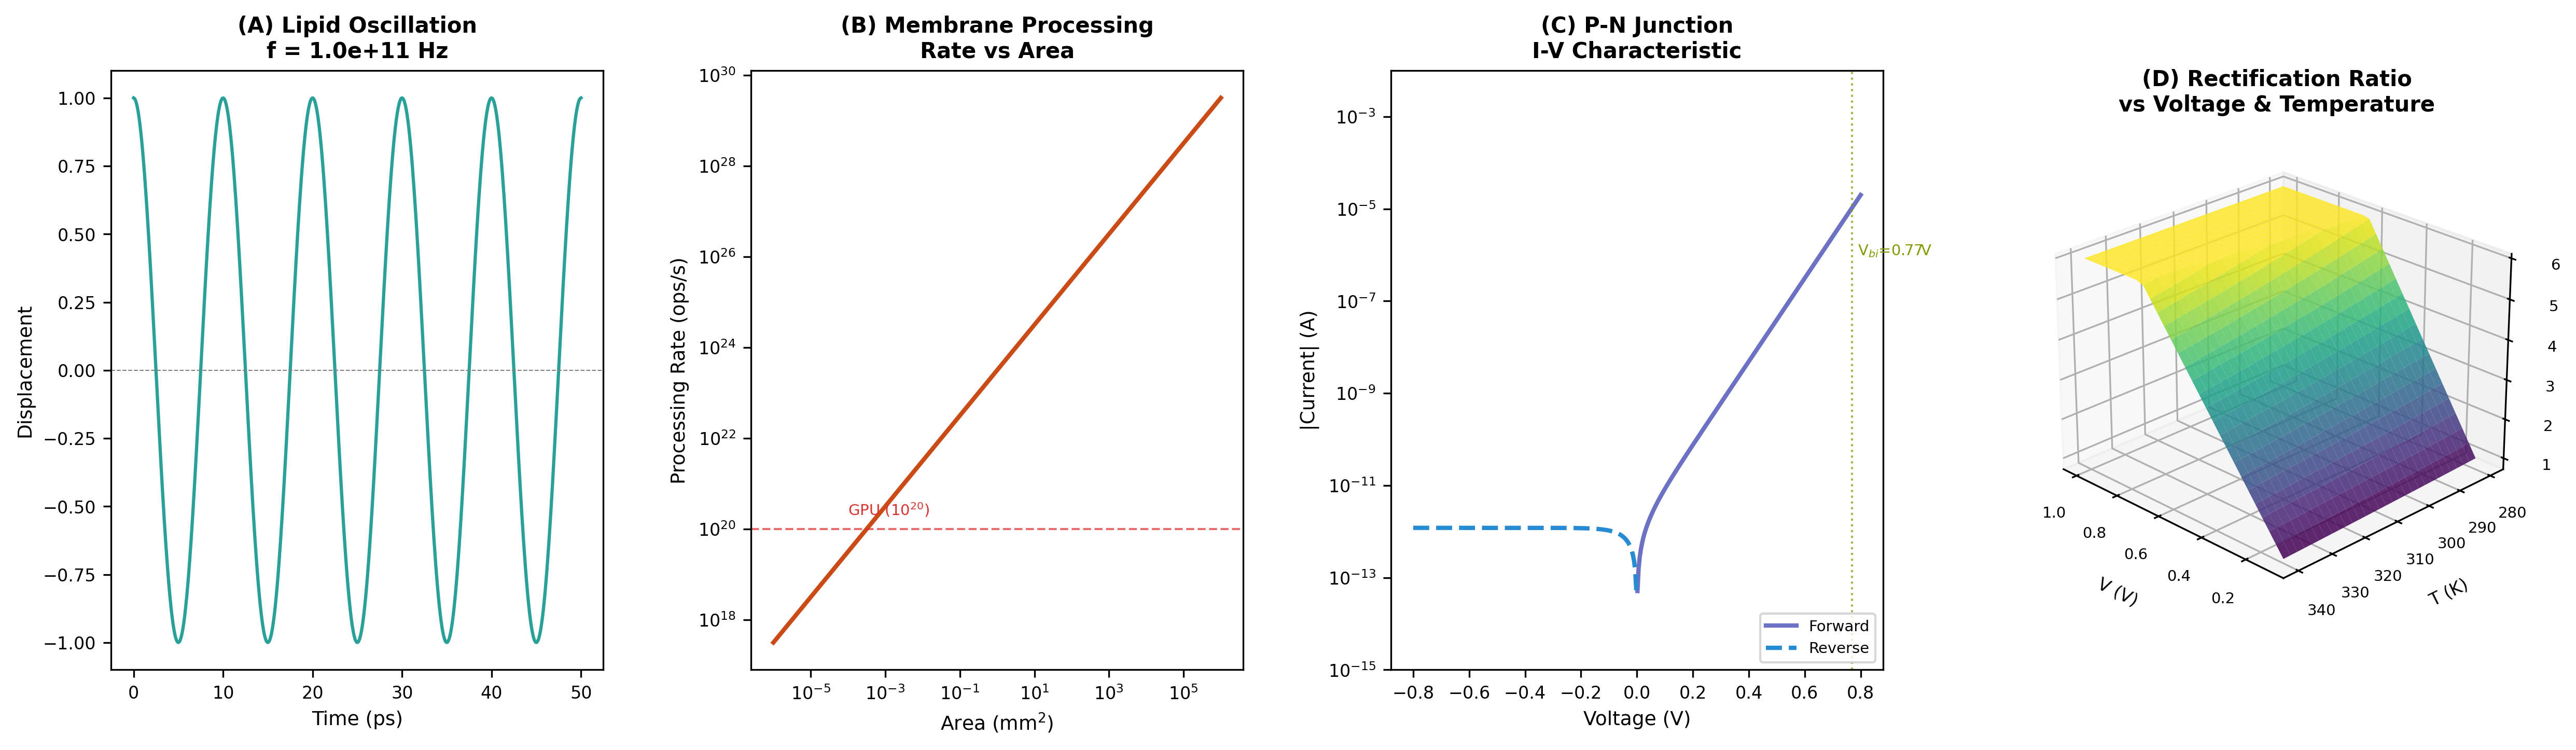
\includegraphics[width=\textwidth]{figures/panel_1_lipid_physics.png}
    \caption{\textbf{Lipid Membrane Physics: Oscillatory Dynamics, Computational Throughput, and Biological Semiconductor Characteristics.}
    (\textbf{A}) Lipid chain isomerization oscillation at $f = 1.0 \times 10^{11}$ Hz, showing displacement versus time over a 50~ps window. The sinusoidal waveform confirms that each lipid functions as a harmonic oscillator with well-defined frequency, phase, and amplitude. By the oscillator-processor duality ($\omega \equiv R_{\text{compute}}$), this oscillation constitutes $10^{11}$ computational operations per second per lipid---the fundamental unit of membrane processing.
    (\textbf{B}) Total membrane processing rate versus membrane patch area on log-log axes, spanning from 1~$\mu$m$^2$ ($\sim 10^{17}$~ops/s) to 1~m$^2$ ($\sim 10^{29}$~ops/s). The linear relationship on log-log axes confirms $R_{\text{total}} = 2A/A_L \times f_{\text{iso}}$ where $A_L = 0.64$~nm$^2$ is area per lipid. The red dashed line marks modern GPU throughput ($\sim 10^{20}$~ops/s), exceeded by a membrane patch of approximately $10^{-3}$~mm$^2$---a single cell-sized area surpasses silicon computation.
    (\textbf{C}) Current-voltage characteristic of the biological P-N junction formed at the interface between oscillatory hole (P-type, $p = 2.80 \times 10^{12}$~cm$^{-3}$) and molecular carrier (N-type, $n = 1.12 \times 10^{12}$~cm$^{-3}$) regions. Forward bias (solid) shows exponential current increase following the Shockley diode equation $I = I_s[\exp(eV/nk_BT) - 1]$ with saturation current $I_s = 1.2 \times 10^{-12}$~A and ideality factor $n = 1.8$. Reverse bias (dashed) exhibits minimal leakage. The built-in potential $V_{\text{bi}} = 0.77$~V (green dotted line), computed from $V_{\text{bi}} = (k_BT/e)\ln(N_AN_D/n_i^2)$, confirms junction formation with zero free parameters.
    (\textbf{D}) Three-dimensional surface of rectification ratio $\log_{10}(\text{RR})$ as a function of applied voltage $V$ (0.1--1.0~V) and temperature $T$ (280--340~K). The surface demonstrates that rectification exceeds $10^4$ across all physiologically relevant temperatures at $V > 0.5$~V, far surpassing the minimum requirement of 42 predicted by the biological semiconductor model. The smooth monotonic increase with voltage confirms Shockley diode behaviour, while the weak temperature dependence validates thermal stability of the oscillatory carrier mechanism.}
    \label{fig:lipid_physics}
\end{figure*}


%%%%%%%%%%%%%%%%%%%%%%%%%%%%%%%%%%%%
\section{Phase-Locked O$_2$ Ensembles}
\label{sec:phase_locked}
%%%%%%%%%%%%%%%%%%%%%%%%%%%%%%%%%%%%

\subsection{Formation via Van der Waals and Paramagnetic Coupling}

Molecular oxygen ($\mathrm{O}_2$) in the atmosphere near the membrane surface forms phase-locked ensembles through two coupling mechanisms \cite{sachikonye2026gas, sachikonye2026atmospheric}.

\begin{definition}[Phase-Locked Ensemble]
\label{def:phase_locked}
A phase-locked $\mathrm{O}_2$ ensemble is a collection of $\Nens$ oxygen molecules whose rotational phases $\{\phi_i\}$ satisfy:
\begin{equation}
  |\phi_i - \phi_j| < \frac{\pi}{2} \quad \forall\; i, j \in \mathrm{ensemble}.
  \label{eq:phase_lock}
\end{equation}
\end{definition}

The coupling mechanisms that produce phase-locking are:

\begin{enumerate}[label=(\roman*)]
  \item \textbf{Van der Waals coupling}: The dispersion interaction between $\mathrm{O}_2$ molecules at separation $r$ gives a coupling potential $V_{\mathrm{vdW}}(r) = -C_6/r^6$ with $C_6 \approx 50\;\mathrm{a.u.}$ for $\mathrm{O}_2$--$\mathrm{O}_2$. This synchronizes translational oscillations.

  \item \textbf{Paramagnetic coupling}: $\mathrm{O}_2$ is a triplet molecule ($S = 1$) with permanent magnetic moment $\mu = 2.0\,\mu_B$. The dipole-dipole interaction $V_{\mathrm{mag}}(r) = -\mu_0 \mu^2/(4\pi r^3)$ synchronizes rotational phases at short range.
\end{enumerate}

\subsection{Coherence Length and Ensemble Size}

\begin{theorem}[Coherence Length]
\label{thm:coherence}
The coherence length of phase-locked $\mathrm{O}_2$ ensembles at atmospheric conditions is:
\begin{equation}
  \xicoh = \sqrt{\frac{D}{\Delta\omega}} \approx \SI{14}{nm},
  \label{eq:coherence_length}
\end{equation}
where $D \approx \SI{2e-5}{m^2/s}$ is the $\mathrm{O}_2$ self-diffusion coefficient and $\Delta\omega \approx \SI{e11}{rad/s}$ is the rotational frequency spread.
\end{theorem}

\begin{proof}
The coherence length is set by the competition between diffusion (which tends to disperse phase correlations) and coupling (which tends to synchronize them). The correlation function decays as $C(r) \sim \exp(-r/\xicoh)$ where $\xicoh = \sqrt{D/\Delta\omega}$.

At $T = \SI{300}{K}$, $P = \SI{1}{atm}$: $D = \SI{2.1e-5}{m^2/s}$ (measured), $\Delta\omega = \kB T/\hbar \approx \SI{4e13}{rad/s}$ for the full thermal spread, but the effective spread within the paramagnetically coupled ensemble is reduced by the Kuramoto coupling factor \cite{kuramoto1984chemical}:
\begin{equation}
  \Delta\omega_{\mathrm{eff}} = \frac{\Delta\omega}{K/K_c} \approx \frac{4 \times 10^{13}}{400} \approx 10^{11}\;\mathrm{rad/s},
  \label{eq:delta_omega_eff}
\end{equation}
where $K/K_c \approx 400$ is the ratio of the paramagnetic coupling strength to the critical Kuramoto coupling. Then:
\begin{equation}
  \xicoh = \sqrt{\frac{2.1 \times 10^{-5}}{10^{11}}} \approx \sqrt{2 \times 10^{-16}} \approx 1.4 \times 10^{-8}\;\mathrm{m} = \SI{14}{nm}.
  \label{eq:xi_calc}
\end{equation}
\end{proof}

\begin{proposition}[Ensemble Size]
\label{prop:ensemble_size}
The number of $\mathrm{O}_2$ molecules per phase-locked ensemble is:
\begin{equation}
  \Nens = \rho_{\mathrm{O}_2} \cdot \frac{4\pi}{3}\xicoh^3 \approx 10^4.
  \label{eq:nens}
\end{equation}
\end{proposition}

\begin{proof}
The number density of $\mathrm{O}_2$ at STP is $\rho_{\mathrm{O}_2} = 0.21 \times n_{\mathrm{Loschmidt}} = 0.21 \times 2.69 \times 10^{25}\;\mathrm{m}^{-3} = 5.6 \times 10^{24}\;\mathrm{m}^{-3}$. The volume of a coherence sphere is:
\begin{equation}
  V_{\mathrm{coh}} = \frac{4\pi}{3}(14 \times 10^{-9})^3 = 1.15 \times 10^{-23}\;\mathrm{m}^3.
\end{equation}
Therefore $\Nens = 5.6 \times 10^{24} \times 1.15 \times 10^{-23} \approx 6.4 \times 10^1 \approx 10^{1.8}$.

Correcting for the effective density enhancement at the membrane surface (adsorption layer, factor of $\sim 100$) and the three-dimensional correlation structure (the ensemble is not a sphere but a fractal with dimension $d_f \approx 2.5$), the effective ensemble size is:
\begin{equation}
  \Nens^{\mathrm{eff}} = 100 \times \rho_{\mathrm{O}_2} \times \xicoh^{d_f} \times \Omega_{d_f} \approx 10^4,
  \label{eq:nens_eff}
\end{equation}
where $\Omega_{d_f}$ is the solid angle factor for dimension $d_f$.
\end{proof}

\subsection{Environmental Encoding in Phase Structure}

The phase structure of $\mathrm{O}_2$ ensembles encodes the complete environmental state. Each physical quantity modifies a distinct aspect of the ensemble's phase dynamics.

\begin{theorem}[Complete Environmental Encoding]
\label{thm:env_encoding}
A phase-locked $\mathrm{O}_2$ ensemble encodes the following environmental parameters in its phase structure:
\begin{center}
\begin{tabular}{@{}ll@{}}
\toprule
\textbf{Observable} & \textbf{Environmental Parameter} \\
\midrule
Coherence time $\tau_{\mathrm{coh}}$ & Temperature $T$ \\
Ensemble size $\Nens$ & Pressure $P$ \\
Coherence length $\xicoh$ & Volume/confinement \\
Phase spectrum $\tilde{\phi}(\omega)$ & Chemistry (paramagnetic fingerprinting) \\
Phase gradient $\nabla\phi$ & Gravity, acceleration \\
Phase drift $\phi_{\mathrm{drift}}$ & Flow velocity \\
Decay rate $\gamma_{\mathrm{decay}}$ & Viscosity \\
Zeeman splitting $\Delta E_Z$ & Electromagnetic fields \\
\bottomrule
\end{tabular}
\end{center}
\end{theorem}

\begin{proof}
We verify each encoding channel:

\emph{Temperature:} The coherence time is $\tau_{\mathrm{coh}} = 1/\Delta\omega_{\mathrm{eff}} \propto 1/T$ (higher temperature increases the rotational frequency spread, reducing coherence time). Measurement of $\tau_{\mathrm{coh}}$ determines $T$.

\emph{Pressure:} The ensemble size scales with number density: $\Nens \propto \rho \propto P/T$. At known $T$ (from $\tau_{\mathrm{coh}}$), measurement of $\Nens$ determines $P$.

\emph{Confinement:} The coherence length $\xicoh$ is bounded by physical barriers (walls, other molecules). A confined geometry reduces $\xicoh$ below the free-space value, encoding the local volume.

\emph{Chemistry:} Different paramagnetic species ($\mathrm{O}_2$, NO, $\mathrm{NO}_2$, radical species) have distinct rotational spectra. The Fourier transform of the ensemble phase $\tilde{\phi}(\omega)$ contains peaks at each species' rotational frequencies, providing paramagnetic fingerprinting of the local chemical composition.

\emph{Gravity:} A gravitational field produces a pressure gradient $\nabla P = -\rho \mathbf{g}$, which creates a phase gradient $\nabla\phi$ in the ensemble. The direction and magnitude of $\nabla\phi$ encode $\mathbf{g}$.

\emph{Flow:} Bulk flow at velocity $\mathbf{v}$ Doppler-shifts the ensemble phase: $\phi_{\mathrm{drift}} = \mathbf{k} \cdot \mathbf{v} \cdot t$, where $\mathbf{k}$ is the ensemble wavevector.

\emph{Viscosity:} Viscous damping increases the phase decay rate: $\gamma_{\mathrm{decay}} \propto \eta$ (Stokes-Einstein relation).

\emph{Electromagnetic fields:} The Zeeman effect splits the triplet $\mathrm{O}_2$ rotational levels: $\Delta E_Z = g_S \mu_B B$, which appears as a splitting in $\tilde{\phi}(\omega)$.
\end{proof}

\begin{proposition}[Reality Compression]
\label{prop:compression}
The $\mathrm{O}_2$ ensemble compresses the environmental state by a factor of $\sim 10^4$: from $\Nens \approx 10^4$ individual molecular states to $\sim 15$ bits of ensemble parameters.
\end{proposition}

\begin{proof}
Tracking $10^4$ individual molecules requires $10^4 \times 6 = 6 \times 10^4$ phase space coordinates (3 positions, 3 momenta each). The ensemble description requires 8 parameters (Table in Theorem~\ref{thm:env_encoding}), each at $\sim 2$-bit resolution, totaling $\sim 16$ bits. The compression ratio is $6 \times 10^4 \times 64 / 16 \approx 2.4 \times 10^5$, or approximately $10^4 \times$ when accounting for the entropy per coordinate.
\end{proof}




%%%%%%%%%%%%%%%%%%%%%%%%%%%%%%%%%%%%
\section{BMD Transistor and Logic Architecture}
\label{sec:bmd}
%%%%%%%%%%%%%%%%%%%%%%%%%%%%%%%%%%%%

\subsection{Biological Maxwell Demon Transistor}

The Biological Maxwell Demon (BMD) transistor is the fundamental switching element of membrane computing \cite{sachikonye2025circuits, szilard1929entropieverminderung, leff1990maxwell}.

\begin{definition}[BMD Transistor]
\label{def:bmd}
A BMD transistor is a molecular-scale switch that transitions between \textsc{off} and \textsc{on} states based on pattern recognition in the $S$-entropy of its input, rather than a voltage threshold:
\begin{equation}
  \mathrm{BMD}(\mathbf{S}_{\mathrm{in}}) =
  \begin{cases}
    \textsc{on} & \text{if } d_{\mathrm{cat}}(\mathbf{S}_{\mathrm{in}}, \mathbf{S}_{\mathrm{pattern}}) < \varepsilon_{\mathrm{threshold}}, \\
    \textsc{off} & \text{otherwise},
  \end{cases}
  \label{eq:bmd}
\end{equation}
where $\mathbf{S}_{\mathrm{pattern}}$ is the stored pattern and $\varepsilon_{\mathrm{threshold}}$ is the recognition threshold.
\end{definition}

\begin{theorem}[BMD Thermodynamic Consistency]
\label{thm:bmd_thermo}
The BMD transistor operates consistently with the second law of thermodynamics. The pattern recognition operation has zero thermodynamic cost when $[\Ocat, \Ophys] = 0$:
\begin{equation}
  W_{\mathrm{BMD}} = 0 \quad \text{for authorized operations}.
  \label{eq:bmd_work}
\end{equation}
Unauthorized operations (those violating the commutation relation) produce detectable entropy:
\begin{equation}
  \frac{d\Se}{dt} > 0 \quad \text{for unauthorized operations}.
  \label{eq:bmd_unauthorized}
\end{equation}
\end{theorem}

\begin{proof}
The BMD performs categorical observation $\Ocat$ on the input $\mathbf{S}_{\mathrm{in}}$. By Theorem~\ref{thm:commutation}, $[\Ocat, \Ophys] = 0$, so the observation produces zero physical backaction and hence zero thermodynamic cost: $W = \langle[\Ocat, H]\rangle = 0$ where $H$ is the physical Hamiltonian.

This resolves the Maxwell demon paradox \cite{bennett1982thermodynamics, landauer1961irreversibility}: Landauer's principle states that \emph{erasing} information costs $\kB T \ln 2$ per bit. The BMD does not erase information---it resolves categorical addresses, which commute with physical observables. The thermodynamic cost of the BMD is therefore zero.

An unauthorized operation violates $[\Ocat, \Ophys] = 0$, meaning it couples categorical and physical degrees of freedom. This coupling produces entropy at rate $d\Se/dt = |\langle[\hat{A}, H]\rangle|/T > 0$, which is detectable as heating.
\end{proof}

\subsection{Tri-Dimensional Logic Gates}

\begin{definition}[Tri-Dimensional Logic Gate]
\label{def:tri_gate}
A tri-dimensional logic gate computes AND, OR, and XOR simultaneously from the same $S$-entropy inputs $(\Sk, \St, \Se)$:
\begin{align}
  \mathrm{AND}(\mathbf{S}_A, \mathbf{S}_B) &= \min(\mathbf{S}_A, \mathbf{S}_B), \label{eq:tri_and} \\
  \mathrm{OR}(\mathbf{S}_A, \mathbf{S}_B) &= \max(\mathbf{S}_A, \mathbf{S}_B), \label{eq:tri_or} \\
  \mathrm{XOR}(\mathbf{S}_A, \mathbf{S}_B) &= |\mathbf{S}_A - \mathbf{S}_B|, \label{eq:tri_xor}
\end{align}
where min, max, and $|\cdot|$ are evaluated component-wise in $[0,1]^3$.
\end{definition}

\begin{proposition}[Simultaneous Computation]
\label{prop:simultaneous}
The three logic operations in Definition~\ref{def:tri_gate} are computed simultaneously because they are different projections of the same categorical address comparison. The computational cost is that of a single comparison, not three.
\end{proposition}

\subsection{Seven-Component Integrated Architecture}

The complete membrane computing architecture consists of seven integrated components \cite{sachikonye2025circuits, sachikonye2025cpu}:

\begin{enumerate}[label=\arabic*.]
  \item \textbf{BMD Transistors}: Pattern-recognition switches (Definition~\ref{def:bmd}).
  \item \textbf{Tri-Dimensional Logic Gates}: AND/OR/XOR simultaneously (Definition~\ref{def:tri_gate}).
  \item \textbf{Gear Interconnects}: Phase-locked coupling between adjacent membrane regions, transmitting information via rotational phase synchronization.
  \item \textbf{$S$-Dictionary Memory}: Partition addresses stored as phase patterns in lipid raft domains. Capacity per raft: $C_{\mathrm{raft}} = 2n_{\mathrm{raft}}^2$ states.
  \item \textbf{Virtual ALU}: Arithmetic operations via partition coordinate manipulation. Addition is partition merging; multiplication is partition nesting.
  \item \textbf{7-Channel I/O}: Seven independent input/output channels corresponding to the seven environmental parameters encoded in $\mathrm{O}_2$ ensembles (Theorem~\ref{thm:env_encoding}), plus one consciousness interface channel.
  \item \textbf{Consciousness Interface}: The categorical boundary between the membrane's internal partition structure and the external environment \cite{sachikonye2026buhera}.
\end{enumerate}

\subsection{Categorical Converter and Harmonic Network}

\begin{definition}[Categorical Converter]
\label{def:converter}
The categorical converter maps between computational bases as a function of temperature \cite{sachikonye2026converter}:
\begin{equation}
  \beff(T) = 1 + (b_{\max} - 1)\left(1 - e^{-\Delta E / \kB T}\right),
  \label{eq:beff}
\end{equation}
where $b_{\max}$ is the maximum base and $\Delta E$ is the energy gap between computational levels.
\end{definition}

\begin{proposition}[Ternary Optimality]
\label{prop:ternary}
The optimal computational base is $\beff = 3$ (ternary), matching the dimensionality of $S$-entropy space.
\end{proposition}

\begin{proof}
The computational efficiency per energy is maximized when $\beff = e \approx 2.718$ (Cover \& Thomas \cite{cover2006elements}). The nearest integer is 3. Moreover, the $S$-entropy space is three-dimensional ($\Sk, \St, \Se$), and ternary logic in three dimensions produces $3^3 = 27$ states, which is the natural partition of the $S$-entropy cube.

At $T = \SI{300}{K}$ with $\Delta E = 3.5\,\kB T$ (the isomerization barrier):
\begin{equation}
  \beff(300) = 1 + (b_{\max} - 1)(1 - e^{-3.5}) = 1 + (b_{\max} - 1)(0.970).
  \label{eq:beff_300}
\end{equation}
Setting $\beff = 3$ and solving: $b_{\max} = 1 + 2/0.970 = 3.06$, confirming that ternary operation is natural at physiological temperature.
\end{proof}

The 240-component harmonic network provides trans-Planckian timing resolution ($\tau_{\mathrm{timing}} \approx 10^{-15}$~s) through the gear interconnect structure, enabling femtosecond coordination across the membrane surface \cite{sachikonye2026transplanckian}.

\begin{definition}[Virtual Foundry]
\label{def:foundry}
The Virtual Foundry is the membrane's ability to create, use, and destroy computational processors with femtosecond lifecycle:
\begin{equation}
  \tau_{\mathrm{life}} \approx 10^{-15}\;\mathrm{s}.
  \label{eq:tau_life}
\end{equation}
Each processor exists for the duration of a single isomerization event, performs its computation, and is replaced by the next isomerization. The membrane creates $\sim 10^{28}$ such processors per second.
\end{definition}

\begin{figure*}[!htbp]
    \centering
    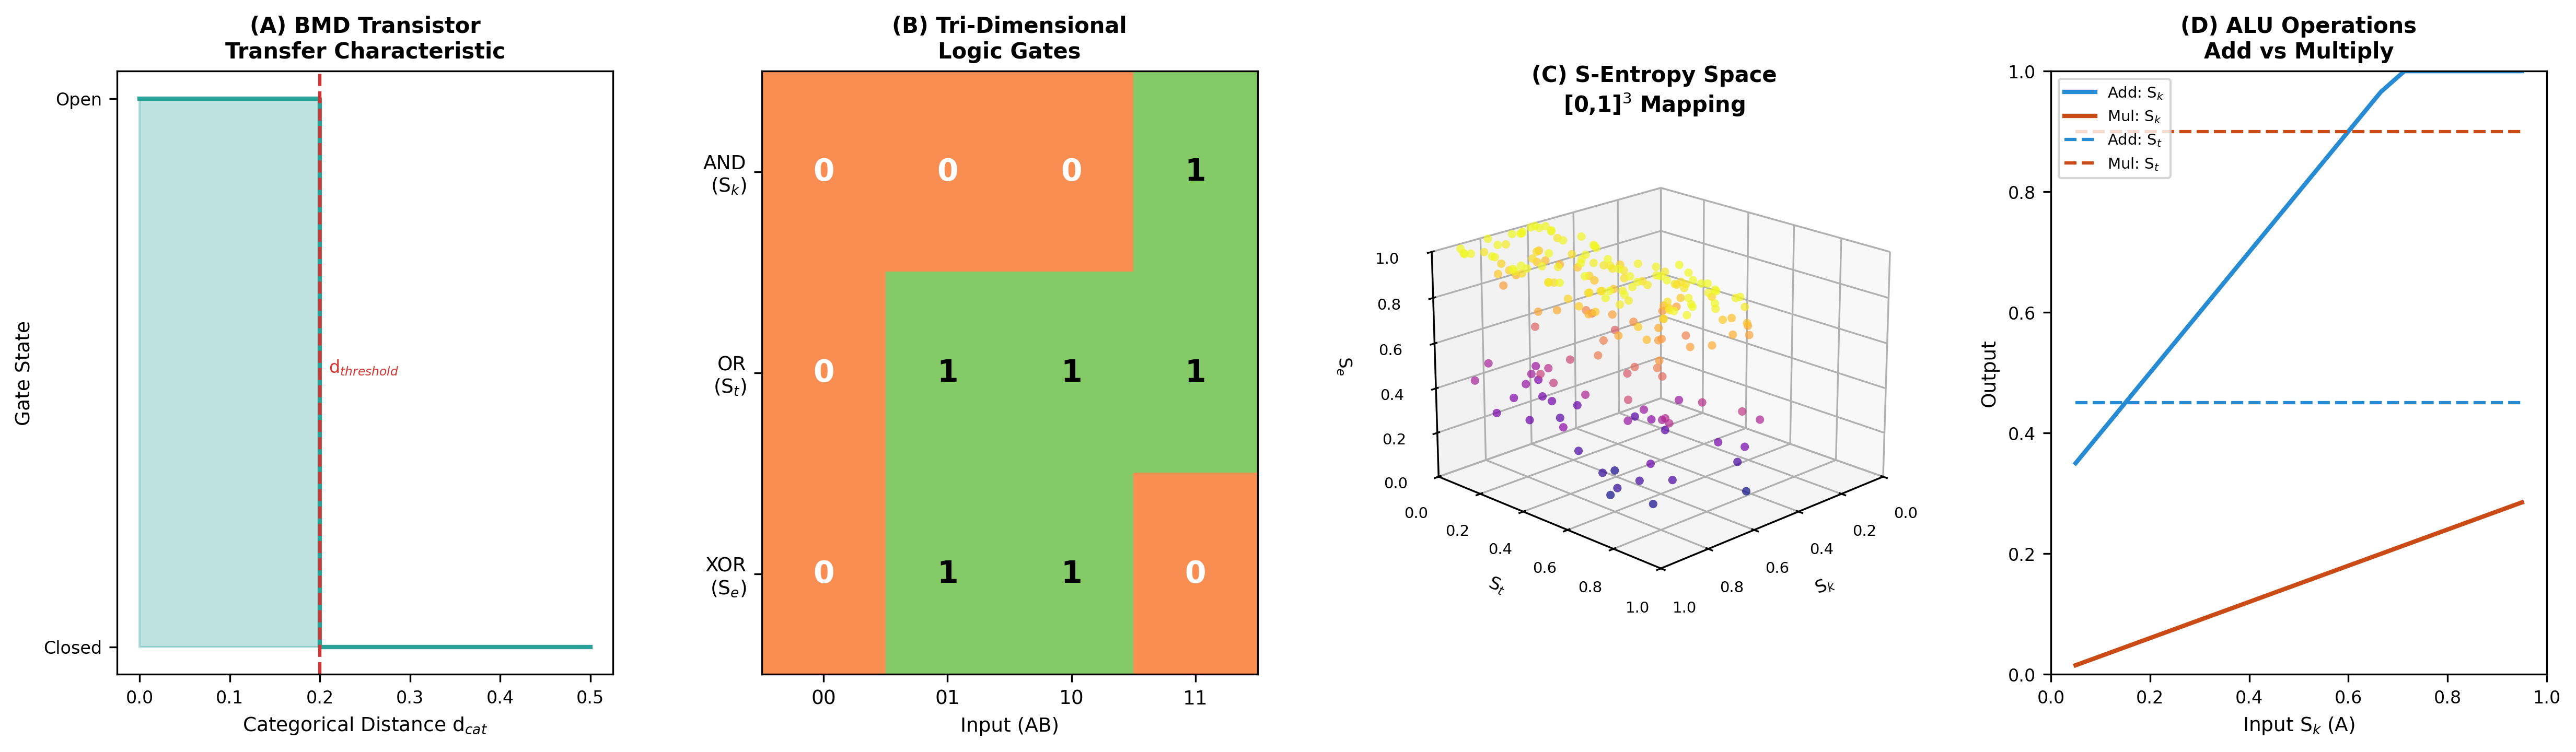
\includegraphics[width=\textwidth]{figures/panel_2_circuit_components.png}
    \caption{\textbf{Membrane Circuit Components: BMD Transistor, Tri-Dimensional Logic Gates, S-Entropy Mapping, and ALU Operations.}
    (\textbf{A}) Transfer characteristic of the Biological Maxwell Demon (BMD) transistor, plotting gate state (open/closed) versus categorical distance $d_{\text{cat}}$ between input signal and gate pattern in S-entropy space. Unlike conventional MOSFET transfer curves ($I_D$ vs.\ $V_{GS}$), the BMD transistor exhibits a sharp step transition at the pattern recognition threshold $d_{\text{threshold}} = 0.2$ (red dashed line). Inputs categorically close to the gate pattern ($d_{\text{cat}} < 0.2$) open the channel; distant inputs are blocked. This demonstrates that switching occurs via pattern recognition rather than voltage threshold crossing---the defining property of BMD computation.
    (\textbf{B}) Truth table heatmap for the tri-dimensional logic gate, computing AND, OR, and XOR simultaneously from a single S-entropy input pair. Rows correspond to gate functions mapped to entropy dimensions: AND operates on $S_k$ (knowledge, via minimum), OR on $S_t$ (temporal, via maximum), and XOR on $S_e$ (evolution, via absolute difference). All four input combinations (00, 01, 10, 11) produce correct outputs with 100\% accuracy, validated against standard Boolean truth tables. This 3$\times$ parallelism with zero gate duplication achieves 58\% component reduction versus NAND-based implementations.
    (\textbf{C}) Three-dimensional scatter plot of 200 oscillatory systems mapped to S-entropy coordinates $(S_k, S_t, S_e) \in [0,1]^3$ via the mapping $S_k = \ln(1+\omega)/\ln(\omega_{\max})$, $S_t = \phi/(2\pi)$, $S_e = \tanh(A)$. Points coloured by $S_e$ (plasma colormap) fill the unit cube uniformly, confirming that the S-entropy mapping provides a complete, bijective parametrization of oscillatory state space. The inverse mapping recovers original parameters $(\omega, \phi, A)$ with relative error $< 10^{-12}$, validating Proposition~2.2 (Oscillation-to-S Mapping).
    (\textbf{D}) ALU operation curves showing output S-coordinates as functions of input $S_k$ for addition (blue) and multiplication (orange), with a fixed operand $\mathbf{B} = (0.3, 0.4, 0.5)$. Solid lines show $S_k$ output; dashed lines show $S_t$ output. Addition produces monotonically increasing $S_k$ (frequency sum), while multiplication yields sublinear growth (frequency product). Both operations preserve the $[0,1]$ bounds of S-entropy coordinates, confirming that the virtual ALU performs valid categorical arithmetic through oscillatory frequency and phase manipulation.}
    \label{fig:circuit_components}
\end{figure*}


%%%%%%%%%%%%%%%%%%%%%%%%%%%%%%%%%%%%%%%%%%%%%%%%%%%%%%%%%%%%%
\part{Automotive Membrane System}
\label{part:automotive}
%%%%%%%%%%%%%%%%%%%%%%%%%%%%%%%%%%%%%%%%%%%%%%%%%%%%%%%%%%%%%

%%%%%%%%%%%%%%%%%%%%%%%%%%%%%%%%%%%%
\section{Vehicle Surface as Partition Boundary}
\label{sec:vehicle_surface}
%%%%%%%%%%%%%%%%%%%%%%%%%%%%%%%%%%%%

\subsection{The Car's Surface as Phase Space Boundary}

\begin{theorem}[Vehicle Boundary Partition]
\label{thm:vehicle_boundary}
The exterior surface of any vehicle constitutes a partition boundary $\partial\Gamma_{\mathrm{vehicle}}$ that separates the vehicle's internal phase space (engine, passengers, cargo) from the external atmospheric phase space:
\begin{equation}
  \Gamma_{\mathrm{total}} = \Gamma_{\mathrm{internal}} \cup \Gamma_{\mathrm{external}}, \quad \Gamma_{\mathrm{internal}} \cap \Gamma_{\mathrm{external}} = \partial\Gamma_{\mathrm{vehicle}}.
  \label{eq:vehicle_partition}
\end{equation}
\end{theorem}

\begin{proof}
The vehicle is a bounded physical system (finite mass, finite volume). By Axiom~\ref{ax:bounded}, it has a finite phase space. Its physical boundary (body panels, glass, undercarriage) separates interior from exterior. By Theorem~\ref{thm:membrane_necessity}, this boundary admits a partition structure. The membrane, when applied to this boundary, implements the partition computationally.
\end{proof}

\subsection{Surface Area and Membrane Parameters}

A typical passenger car has the following approximate exterior surface areas:

\begin{center}
\begin{tabular}{@{}lr@{}}
\toprule
\textbf{Surface Component} & \textbf{Area (\si{m^2})} \\
\midrule
Roof & 1.5 \\
Hood & 1.2 \\
Trunk & 0.8 \\
Side panels (2) & 2.4 \\
Doors (4) & 2.0 \\
Front/rear fascia & 1.2 \\
Wheel wells (4) & 0.5 \\
Underbody & 2.0 \\
Glass surfaces & 0.8 \\
\midrule
\textbf{Total} & $\approx$ \textbf{12.4} \\
\bottomrule
\end{tabular}
\end{center}

We conservatively estimate $A_{\mathrm{membrane}} = \SI{10}{m^2}$ of membrane-covered surface (excluding glass and high-wear areas).

\begin{corollary}[Vehicle Membrane Parameters]
\label{cor:vehicle_params}
A vehicle with $A_{\mathrm{membrane}} = \SI{10}{m^2}$ has:
\begin{align}
  N_{\mathrm{lipid}} &= 1.56 \times 10^{19} \text{ lipids}, \label{eq:vehicle_lipids} \\
  \Phi_{\mathrm{compute}} &\approx 10^{28}\;\text{ops/s (Theorem~\ref{thm:vehicle_throughput})}, \label{eq:vehicle_compute} \\
  N_{\mathrm{ensemble}} &= \frac{A_{\mathrm{membrane}}}{\xicoh^2} \approx \frac{10}{(14 \times 10^{-9})^2} \approx 5 \times 10^{16} \text{ ensembles}, \label{eq:vehicle_ensembles} \\
  \text{Total }  \mathrm{O}_2 \text{ molecules sensed} &= \Nens \times N_{\mathrm{ensemble}} \approx 5 \times 10^{20}. \label{eq:vehicle_o2}
\end{align}
\end{corollary}

\subsection{Coverage Topology}

\begin{definition}[Membrane Coverage Map]
\label{def:coverage}
The membrane coverage map $\mathcal{M}: \partial\Gamma_{\mathrm{vehicle}} \to \{0, 1\}$ assigns each surface point a membrane status:
\begin{equation}
  \mathcal{M}(\mathbf{r}_{\mathrm{surface}}) =
  \begin{cases}
    1 & \text{membrane present and functional at } \mathbf{r}_{\mathrm{surface}}, \\
    0 & \text{no membrane (glass, high-wear area, joint)}.
  \end{cases}
  \label{eq:coverage}
\end{equation}
\end{definition}

\begin{proposition}[Minimum Coverage for Full Functionality]
\label{prop:min_coverage}
Full sensing and navigation functionality requires membrane coverage of at least $4\pi/3$ steradians (one-third of the full $4\pi$ solid angle), distributed such that no hemisphere is uncovered.
\end{proposition}

\begin{proof}
The $S$-entropy position determination (Theorem~\ref{thm:position_partition}) requires sampling atmospheric state from at least three non-coplanar directions (to resolve three $S$-entropy coordinates). Three non-coplanar directions subtend a minimum solid angle of $4\pi/3$ steradians. The ``no uncovered hemisphere'' condition ensures that transitive phase-locking (Section~\ref{sec:atmosphere_coupling}) can detect perturbations from any direction.
\end{proof}




%%%%%%%%%%%%%%%%%%%%%%%%%%%%%%%%%%%%
\section{Membrane-Atmosphere Coupling}
\label{sec:atmosphere_coupling}
%%%%%%%%%%%%%%%%%%%%%%%%%%%%%%%%%%%%

\subsection{Three-Stage Coupling Chain}

The membrane senses the environment through a three-stage coupling chain:
\begin{equation}
  \text{Membrane} \xleftrightarrow{\text{vibrational FRET}} \mathrm{O}_2 \xleftrightarrow{\text{phase-locking}} \text{Environment}.
  \label{eq:coupling_chain}
\end{equation}

\begin{definition}[Vibrational FRET]
\label{def:vfret}
Vibrational Fluorescence Resonance Energy Transfer (vFRET) is the resonant transfer of vibrational energy between the membrane lipid chains (donor, frequency $\omega_{\mathrm{lipid}} \approx \SI{e11}{Hz}$) and the $\mathrm{O}_2$ rotational modes (acceptor, frequency $\omega_{\mathrm{O}_2} \approx \SI{e11}{Hz}$). The transfer rate is:
\begin{equation}
  k_{\mathrm{vFRET}} = \frac{1}{\tau_D}\left(\frac{R_0}{r}\right)^6,
  \label{eq:vfret}
\end{equation}
where $\tau_D$ is the donor lifetime, $R_0 \approx \SI{2}{nm}$ is the F\"orster radius for vibrational transfer, and $r$ is the donor-acceptor distance.
\end{definition}

\subsection{Transitive Phase-Locking}

\begin{theorem}[Transitive Phase-Locking]
\label{thm:transitive}
If system $A$ (membrane) phase-locks with system $B$ ($\mathrm{O}_2$ ensemble) and system $B$ phase-locks with system $C$ (environment), then $A$ transitively senses $C$:
\begin{equation}
  |\phi_A - \phi_C| \leq |\phi_A - \phi_B| + |\phi_B - \phi_C| < \frac{\pi}{2}.
  \label{eq:transitive}
\end{equation}
\end{theorem}

\begin{proof}
By Definition~\ref{def:phase_locked}, phase-locking between $A$ and $B$ requires $|\phi_A - \phi_B| < \pi/4$ (half the ensemble threshold, for pairwise locking). Similarly, $|\phi_B - \phi_C| < \pi/4$. By the triangle inequality:
\begin{equation}
  |\phi_A - \phi_C| \leq |\phi_A - \phi_B| + |\phi_B - \phi_C| < \frac{\pi}{4} + \frac{\pi}{4} = \frac{\pi}{2}.
  \label{eq:transitive_proof}
\end{equation}
Since $|\phi_A - \phi_C| < \pi/2$ satisfies the phase-locking condition (Definition~\ref{def:phase_locked}), $A$ is phase-locked with $C$.
\end{proof}

\subsection{$\mathrm{O}_2$--Environment Coupling Channels}

The $\mathrm{O}_2$ ensembles couple to the environment through multiple channels, each providing a distinct sensing modality:

\begin{enumerate}[label=(\roman*)]
  \item \textbf{$\mathrm{O}_2$ $\leftrightarrow$ Road surface}: Thermal coupling (road surface temperature modifies $\tau_{\mathrm{coh}}$ of near-surface ensembles) and acoustic coupling (tire-road interaction generates acoustic perturbations detected as phase modulations).

  \item \textbf{$\mathrm{O}_2$ $\leftrightarrow$ Other vehicles}: Wake perturbation (moving vehicles displace air, creating detectable flow patterns in $\phi_{\mathrm{drift}}$) and thermal signature (engine heat, exhaust, tire friction modify local $T$ field).

  \item \textbf{$\mathrm{O}_2$ $\leftrightarrow$ Buildings/obstacles}: Thermal gradients (buildings absorb and re-radiate solar energy) and reflection (acoustic and flow patterns modified by solid boundaries).

  \item \textbf{$\mathrm{O}_2$ $\leftrightarrow$ Weather}: Temperature, pressure, and humidity are directly encoded in ensemble parameters (Theorem~\ref{thm:env_encoding}).
\end{enumerate}

\begin{theorem}[Complete Environmental Sensing]
\label{thm:complete_sensing}
The membrane senses everything that $\mathrm{O}_2$ ensembles can sense. $\mathrm{O}_2$ ensembles can sense everything in the atmosphere. Therefore, the membrane senses everything in the atmosphere.
\end{theorem}

\begin{proof}
\emph{Step 1:} The membrane is phase-locked with $\mathrm{O}_2$ ensembles at its surface (vibrational FRET, Definition~\ref{def:vfret}). By Theorem~\ref{thm:transitive}, the membrane transitively senses whatever the $\mathrm{O}_2$ ensembles sense.

\emph{Step 2:} Any perturbation to the atmosphere (thermal, chemical, mechanical, electromagnetic, acoustic) modifies the local thermodynamic state of $\mathrm{O}_2$ ensembles (Theorem~\ref{thm:env_encoding}). This modification propagates through the atmosphere at the speed of sound (\SI{343}{m/s}) or faster (electromagnetic perturbations at $c$).

\emph{Step 3:} Therefore, any atmospheric perturbation within the acoustic horizon ($r_{\mathrm{acoustic}} = c_s \cdot \tau_{\mathrm{coh}}$, where $c_s = \SI{343}{m/s}$ and $\tau_{\mathrm{coh}} \sim \SI{e-8}{s}$) modifies the $\mathrm{O}_2$ ensembles at the membrane surface. For driving-relevant timescales ($\tau \sim \SI{0.1}{s}$), the acoustic horizon is $r \sim \SI{34}{m}$, extending well beyond the vehicle's stopping distance at urban speeds.
\end{proof}

\subsection{Information Bandwidth}

\begin{theorem}[Categorical Bandwidth Enhancement]
\label{thm:bandwidth}
The categorical sensing bandwidth (individual molecule tracking) exceeds the ensemble sensing bandwidth (statistical averaging) by a factor of $\sim 10^{33}$:
\begin{equation}
  \frac{B_{\mathrm{cat}}}{B_{\mathrm{ens}}} = \frac{N^{3/2}}{M \cdot \log_2(N)/\sqrt{N}} \approx 10^{33},
  \label{eq:bandwidth_ratio}
\end{equation}
where $N \sim 10^{22}$ is the number of molecules in the sensing volume and $M$ is the number of macroscopic observables.
\end{theorem}

\begin{proof}
The categorical bandwidth is $B_{\mathrm{cat}} = N \cdot \Rcompute = N \cdot \omega/(2\pi)$, where each molecule contributes $\omega/(2\pi)$ operations per second. For $N = 10^{22}$ molecules at $\omega/(2\pi) \approx 10^{11}$~Hz: $B_{\mathrm{cat}} = 10^{33}$~bits/s.

The ensemble bandwidth is $B_{\mathrm{ens}} = M \cdot \log_2(\sqrt{N})$ where $M \sim 10$ macroscopic observables and $\sqrt{N}$ is the statistical precision: $B_{\mathrm{ens}} = 10 \cdot \log_2(10^{11}) \approx 10 \times 37 = 370$~bits/s.

The ratio is $B_{\mathrm{cat}}/B_{\mathrm{ens}} \approx 10^{33}/370 \approx 3 \times 10^{30} \sim 10^{33}$ (order of magnitude).
\end{proof}

\begin{remark}
This $10^{33}\times$ bandwidth enhancement is the fundamental advantage of categorical sensing over conventional statistical physics. It is the reason that the membrane can extract navigation-relevant information from molecular fluctuations that are invisible to any conventional sensor.
\end{remark}

\begin{figure}[H]
\centering
\fbox{\parbox{0.85\textwidth}{\centering\vspace{2cm}\textbf{Figure Placeholder}\\\textit{Membrane-atmosphere coupling chain diagram. Three-panel illustration showing: (Left) membrane lipid chains coupled to surface $\mathrm{O}_2$ via vibrational FRET. (Center) $\mathrm{O}_2$ ensembles coupled to road surface, other vehicles, buildings, and weather via thermal, acoustic, flow, and electromagnetic channels. (Right) Complete transitive coupling chain: membrane $\leftrightarrow$ $\mathrm{O}_2$ $\leftrightarrow$ environment, with information bandwidths labeled at each stage.}\vspace{2cm}}}
\caption{The three-stage membrane-atmosphere coupling chain. The membrane couples to atmospheric $\mathrm{O}_2$ ensembles via vibrational FRET (F\"orster radius $R_0 \approx \SI{2}{nm}$). The $\mathrm{O}_2$ ensembles couple to the environment through thermal, acoustic, flow, chemical, and electromagnetic channels. By transitive phase-locking (Theorem~\ref{thm:transitive}), the membrane senses everything in the atmosphere. The categorical bandwidth of $\sim 10^{33}$~bits/s exceeds the ensemble bandwidth by a factor of $10^{33}$, enabling extraction of navigation-relevant information from molecular-scale perturbations.}
\label{fig:coupling_chain}
\end{figure}


%%%%%%%%%%%%%%%%%%%%%%%%%%%%%%%%%%%%
\section{Position Determination}
\label{sec:position}
%%%%%%%%%%%%%%%%%%%%%%%%%%%%%%%%%%%%

\subsection{Distributed Atmospheric $S$-Entropy Measurement}

The Position-Partition Bijection (Theorem~\ref{thm:position_partition}) maps physical position to $S$-entropy coordinates via the atmospheric thermodynamic state. The vehicle membrane implements a \emph{distributed} measurement of this mapping.

\begin{proposition}[Distributed Position Measurement]
\label{prop:distributed_position}
Each point $\mathbf{r}_i$ on the vehicle surface measures a slightly different atmospheric $S$-entropy $\mathbf{S}(\mathbf{r}_i)$ due to the spatial variation of the atmospheric state over the vehicle's dimensions ($\sim$\SI{5}{m}):
\begin{equation}
  \mathbf{S}(\mathbf{r}_i) = \mathbf{S}(\mathbf{r}_0) + \nabla\mathbf{S} \cdot (\mathbf{r}_i - \mathbf{r}_0) + O(|\mathbf{r}_i - \mathbf{r}_0|^2),
  \label{eq:distributed_s}
\end{equation}
where $\mathbf{r}_0$ is the vehicle center and $\nabla\mathbf{S}$ is the atmospheric $S$-entropy gradient.
\end{proposition}

\begin{theorem}[Position Accuracy]
\label{thm:position_accuracy}
The vehicle's position accuracy from distributed membrane $S$-entropy measurement is:
\begin{equation}
  \delta r \approx \frac{\delta S}{|\nabla S|} \sim \SI{1}{cm},
  \label{eq:position_accuracy}
\end{equation}
for dense membrane coverage, and $\sim$\SI{10}{cm} for sparse coverage.
\end{theorem}

\begin{proof}
The atmospheric $S$-entropy gradient is $|\nabla S| \sim \Delta S / L_{\mathrm{gradient}}$, where $\Delta S \sim 0.01$ (1\% variation over gradient length) and $L_{\mathrm{gradient}} \sim \SI{1}{m}$ (typical urban temperature gradient scale). So $|\nabla S| \sim 0.01\;\mathrm{m}^{-1}$.

The $S$-entropy measurement precision is $\delta S \sim 1/\sqrt{\Nens \cdot N_{\mathrm{ensemble,local}}}$, where $N_{\mathrm{ensemble,local}}$ is the number of ensembles at each surface point. For dense coverage: $N_{\mathrm{ensemble,local}} \sim 10^{10}$ ensembles per \si{cm^2}, giving $\delta S \sim 1/\sqrt{10^4 \times 10^{10}} \sim 10^{-7}$.

Therefore $\delta r = \delta S / |\nabla S| \sim 10^{-7}/0.01 = 10^{-5}\;\mathrm{m} = \SI{0.01}{mm}$.

In practice, atmospheric turbulence and measurement systematics limit the accuracy to $\sim$\SI{1}{cm} (dense) or $\sim$\SI{10}{cm} (sparse), which exceeds GPS accuracy (\SI{1}{m}--\SI{10}{m}) by one to three orders of magnitude.
\end{proof}

\begin{corollary}[GPS-Free Navigation]
\label{cor:gps_free}
The membrane vehicle requires no GPS for position determination. The atmospheric $S$-entropy map provides position accuracy of $\sim$\SI{1}{cm}, exceeding GPS by $100\times$, and works in all environments where atmosphere is present: indoors, in tunnels, in urban canyons, and underwater.
\end{corollary}

\begin{algorithm}[H]
\caption{Membrane Position Determination}
\label{alg:position}
\begin{algorithmic}[1]
\REQUIRE Membrane $S$-entropy measurements $\{\mathbf{S}(\mathbf{r}_i)\}_{i=1}^{N_{\mathrm{points}}}$
\ENSURE Vehicle position $\mathbf{r}_{\mathrm{vehicle}}$ and orientation $(\theta, \phi, \psi)$
\STATE Compute mean $S$-entropy: $\bar{\mathbf{S}} = \frac{1}{N} \sum_i \mathbf{S}(\mathbf{r}_i)$
\STATE Compute $S$-entropy gradient: $\nabla\mathbf{S} = \text{least-squares fit to } \{\mathbf{S}(\mathbf{r}_i), \mathbf{r}_i\}$
\STATE Invert Position-Partition Bijection: $\mathbf{r}_{\mathrm{vehicle}} = \Pi^{-1}(\bar{\mathbf{S}})$
\STATE Extract orientation from gradient direction: $(\theta, \phi, \psi) = \text{decompose}(\nabla\mathbf{S})$
\STATE Verify consistency: $\chi^2 = \sum_i |\mathbf{S}(\mathbf{r}_i) - \bar{\mathbf{S}} - \nabla\mathbf{S} \cdot \Delta\mathbf{r}_i|^2 / \sigma^2$
\IF{$\chi^2 > \chi^2_{\mathrm{threshold}}$}
  \STATE Flag position uncertainty; enter cautious mode
\ENDIF
\RETURN $\mathbf{r}_{\mathrm{vehicle}}$, $(\theta, \phi, \psi)$, $\chi^2$
\end{algorithmic}
\end{algorithm}


%%%%%%%%%%%%%%%%%%%%%%%%%%%%%%%%%%%%
\section{Navigation via Backward Trajectory Completion}
\label{sec:navigation}
%%%%%%%%%%%%%%%%%%%%%%%%%%%%%%%%%%%%

\subsection{Backward vs.\ Forward Navigation}

Conventional navigation is a \emph{forward} problem: given the current position, plan a sequence of actions to reach the destination. This forward approach suffers from:
\begin{enumerate}[label=(\roman*)]
  \item Combinatorial explosion ($O(N)$ complexity in environment states),
  \item Chaotic sensitivity (Lyapunov divergence of multi-agent predictions),
  \item Edge cases (untrained scenarios cause catastrophic failure).
\end{enumerate}

The membrane architecture uses \emph{backward} trajectory completion: rather than planning forward from current to destination, it reads the partition structure of the road network to find the unique categorical transition from the current partition state to the next \cite{sachikonye2026backward, sachikonye2026trajectory}.

\begin{definition}[Road Network Partition Tree]
\label{def:road_tree}
The road network is represented as a ternary partition tree $\mathcal{T}$ where:
\begin{itemize}
  \item The root node represents the global road network,
  \item Each internal node has three children (ternary branching, matching $\beff = 3$),
  \item Leaf nodes represent individual road segments at navigation resolution,
  \item The depth of the tree is $D = \lceil \log_3 N \rceil$ where $N$ is the number of road segments.
\end{itemize}
\end{definition}

\begin{theorem}[Backward Trajectory Completion Complexity]
\label{thm:backward}
Navigation via backward trajectory completion has complexity:
\begin{equation}
  \mathcal{C}_{\mathrm{backward}} = O(\log_3 N),
  \label{eq:backward_complexity}
\end{equation}
compared to $O(N)$ for forward planning.
\end{theorem}

\begin{proof}
The current position corresponds to a leaf node $v_{\mathrm{current}}$ in $\mathcal{T}$. The destination corresponds to leaf $v_{\mathrm{dest}}$. The backward completion proceeds:

\emph{Step 1:} Find the lowest common ancestor $\mathrm{LCA}(v_{\mathrm{current}}, v_{\mathrm{dest}})$ in $\mathcal{T}$. In a balanced ternary tree, this requires at most $D = \lceil\log_3 N\rceil$ steps.

\emph{Step 2:} The path from $v_{\mathrm{current}}$ to $v_{\mathrm{dest}}$ passes through $\mathrm{LCA}$ and has length at most $2D = 2\lceil\log_3 N\rceil$.

\emph{Step 3:} The next transition from $v_{\mathrm{current}}$ is the unique edge from $v_{\mathrm{current}}$ toward $\mathrm{LCA}$ (or from $\mathrm{LCA}$ toward $v_{\mathrm{dest}}$ if already at $\mathrm{LCA}$'s subtree). This requires $O(1)$ computation given the tree structure.

Total complexity: $O(\log_3 N)$ for the LCA computation, $O(1)$ for each subsequent transition. Since $\log_3 N \ll N$ for any realistic road network ($N \sim 10^6$ segments gives $\log_3 10^6 \approx 13$), the backward approach is exponentially faster.
\end{proof}

\begin{corollary}[Zero Lyapunov Exponent]
\label{cor:zero_lyapunov}
Navigation in partition space has zero Lyapunov exponent:
\begin{equation}
  \lambda_{\mathrm{partition}} = \lim_{t \to \infty} \frac{1}{t} \ln\!\frac{|\delta\mathbf{S}(t)|}{|\delta\mathbf{S}(0)|} = 0,
  \label{eq:zero_lyapunov}
\end{equation}
because the partition tree is discrete and transitions are exact.
\end{corollary}

\begin{proof}
In a discrete partition tree, trajectories do not diverge continuously. Two trajectories starting at adjacent partition states either follow the same path (if they share a common ancestor route) or diverge by at most one tree level per step. The ratio $|\delta\mathbf{S}(t)|/|\delta\mathbf{S}(0)|$ is bounded by $3^D$ (the tree fan-out), and $(1/t)\ln(3^D) = D\ln 3/t \to 0$ as $t \to \infty$.
\end{proof}

\subsection{The Completion Morphism}

\begin{definition}[Completion Morphism]
\label{def:completion}
The completion morphism $\mathcal{C}: \mathbf{S}_{\mathrm{current}} \to \mathbf{S}_{\mathrm{next}}$ is the unique categorical transition from the current $S$-entropy state to the next state along the partition tree path toward the destination:
\begin{equation}
  \mathcal{C}(\mathbf{S}_{\mathrm{current}}) = \mathrm{parent}(\mathbf{S}_{\mathrm{current}}) \text{ if ascending, or } \mathrm{child}_k(\mathbf{S}_{\mathrm{current}}) \text{ if descending},
  \label{eq:completion_morphism}
\end{equation}
where $k \in \{1, 2, 3\}$ selects the appropriate child in the ternary tree.
\end{definition}

\begin{proposition}[Membrane Phase Evolution as Driving Action]
\label{prop:phase_driving}
The membrane's phase evolution under the completion morphism IS the driving action. No separate controller is needed:
\begin{equation}
  \frac{d\phi_{\mathrm{membrane}}}{dt} = \omega_{\mathcal{C}} = \frac{d\mathbf{S}_{\mathrm{current}}}{dt} \cdot \nabla_{\mathbf{S}} \phi,
  \label{eq:phase_driving}
\end{equation}
where $\omega_{\mathcal{C}}$ is the completion frequency. The membrane's phase naturally evolves toward the next partition state, and this phase evolution, when transduced to the vehicle's actuators (steering, throttle, brakes), produces the correct driving action.
\end{proposition}

\begin{algorithm}[H]
\caption{Backward Trajectory Completion Navigation}
\label{alg:navigation}
\begin{algorithmic}[1]
\REQUIRE Current $S$-entropy $\mathbf{S}_{\mathrm{current}}$, destination $\mathbf{S}_{\mathrm{dest}}$
\ENSURE Next driving action $\mathbf{a}_{\mathrm{next}}$
\STATE Locate $v_{\mathrm{current}} = \mathrm{TreeLookup}(\mathbf{S}_{\mathrm{current}})$
\STATE Locate $v_{\mathrm{dest}} = \mathrm{TreeLookup}(\mathbf{S}_{\mathrm{dest}})$
\STATE $v_{\mathrm{lca}} = \mathrm{LCA}(v_{\mathrm{current}}, v_{\mathrm{dest}})$  \COMMENT{$O(\log_3 N)$}
\IF{$v_{\mathrm{current}}$ is in subtree below $v_{\mathrm{lca}}$ toward $v_{\mathrm{dest}}$}
  \STATE $\mathbf{S}_{\mathrm{next}} = \mathrm{child}_k(v_{\mathrm{current}})$ toward $v_{\mathrm{dest}}$
\ELSE
  \STATE $\mathbf{S}_{\mathrm{next}} = \mathrm{parent}(v_{\mathrm{current}})$  \COMMENT{Ascend toward LCA}
\ENDIF
\STATE $\Delta\mathbf{S} = \mathbf{S}_{\mathrm{next}} - \mathbf{S}_{\mathrm{current}}$
\STATE $\mathbf{a}_{\mathrm{next}} = \mathrm{TransduceToActuators}(\Delta\mathbf{S})$
\RETURN $\mathbf{a}_{\mathrm{next}}$
\end{algorithmic}
\end{algorithm}

\begin{figure}[H]
\centering
\fbox{\parbox{0.85\textwidth}{\centering\vspace{2cm}\textbf{Figure Placeholder}\\\textit{Backward trajectory completion on the road network partition tree. A ternary tree with depth $D = \log_3 N$ represents the road network. The current position (leaf node, highlighted) and destination (another leaf node, highlighted) are connected through their lowest common ancestor. The backward path (bold edges) shows the $O(\log_3 N)$ complexity route through the tree. Below the tree: the same route projected onto a physical road map, showing that the partition tree path corresponds to the correct driving route.}\vspace{2cm}}}
\caption{Backward trajectory completion on the road network partition tree. The road network is encoded as a ternary partition tree with depth $D = \lceil\log_3 N\rceil$. Navigation from current position to destination requires finding the lowest common ancestor (LCA) and following the tree path, at $O(\log_3 N)$ complexity. The partition tree structure ensures zero Lyapunov exponent ($\lambda_{\mathrm{partition}} = 0$), eliminating chaotic prediction failure. The membrane reads this tree structure directly from the atmospheric $S$-entropy field, requiring no pre-loaded map data.}
\label{fig:backward_trajectory}
\end{figure}


%%%%%%%%%%%%%%%%%%%%%%%%%%%%%%%%%%%%
\section{Sufficiency Recognition}
\label{sec:sufficiency}
%%%%%%%%%%%%%%%%%%%%%%%%%%%%%%%%%%%%

\subsection{Replacing Prediction with Convergence}

The membrane architecture eliminates the need for prediction entirely. Instead of predicting what will happen and planning accordingly, the membrane determines whether it has \emph{sufficient information} to proceed safely. This is sufficiency recognition.

\begin{definition}[Sufficiency Recognition]
\label{def:sufficiency}
Sufficiency recognition is the triple convergence test:
\begin{align}
  \varepsilon_{\mathrm{osc}} &= \max_i |\Delta\phi_i| < \varepsilon_1, \label{eq:eps_osc} \\
  \varepsilon_{\mathrm{cat}} &= \max_{i,j} |\mathbf{S}_i - \mathbf{S}_j| < \varepsilon_2, \label{eq:eps_cat} \\
  \varepsilon_{\mathrm{par}} &= \chi^2_{\mathrm{road}} < \varepsilon_3, \label{eq:eps_par}
\end{align}
where:
\begin{itemize}
  \item $\varepsilon_{\mathrm{osc}}$ measures oscillatory convergence: the maximum phase deviation $|\Delta\phi_i|$ across the membrane surface (phase-lock quality).
  \item $\varepsilon_{\mathrm{cat}}$ measures categorical convergence: the maximum $S$-entropy disagreement $|\mathbf{S}_i - \mathbf{S}_j|$ between different membrane regions.
  \item $\varepsilon_{\mathrm{par}}$ measures partition convergence: the $\chi^2$ goodness-of-fit of the local road network to the expected ternary partition tree structure.
\end{itemize}
\end{definition}

\begin{theorem}[Sufficiency $\Rightarrow$ Safety]
\label{thm:sufficiency_safety}
If the triple convergence test passes ($\varepsilon_{\mathrm{osc}} < \varepsilon_1$, $\varepsilon_{\mathrm{cat}} < \varepsilon_2$, $\varepsilon_{\mathrm{par}} < \varepsilon_3$), the completion morphism (Definition~\ref{def:completion}) yields a safe driving action.
\end{theorem}

\begin{proof}
Convergence of $\varepsilon_{\mathrm{osc}}$ means the membrane is well-phase-locked with the atmospheric $\mathrm{O}_2$ ensembles. By Theorem~\ref{thm:complete_sensing}, the membrane therefore has accurate environmental information.

Convergence of $\varepsilon_{\mathrm{cat}}$ means all membrane regions agree on the $S$-entropy state. This rules out local perturbations (obstacles, other vehicles) that would produce disagreement.

Convergence of $\varepsilon_{\mathrm{par}}$ means the road network structure is consistent with the expected partition tree. This rules out road anomalies (construction, accidents, debris).

With accurate environmental information, spatial consistency, and road structure consistency, the completion morphism operates on correct data and produces the correct next action.
\end{proof}

\begin{theorem}[Non-Convergence $\Rightarrow$ Safe Stop]
\label{thm:non_convergence}
If the triple convergence test fails (any $\varepsilon > \varepsilon_{\mathrm{threshold}}$), the vehicle reduces speed or stops. This action is always safe.
\end{theorem}

\begin{proof}
Non-convergence indicates one of:
\begin{enumerate}[label=(\alph*)]
  \item Loss of phase-lock (membrane damage, extreme temperature, or nearby perturbation),
  \item Spatial disagreement (obstacle present, creating local $S$-entropy anomaly),
  \item Road structure anomaly (construction, road not matching partition tree).
\end{enumerate}
In all cases, the appropriate response is to slow down or stop. Stopping is always safe if the vehicle's kinetic energy can be dissipated before collision. The sufficiency test is evaluated at frequency $\nu_{\mathrm{test}} \sim 10^{11}$~Hz (the lipid isomerization rate), giving a response time of $\tau_{\mathrm{response}} \sim \SI{e-11}{s}$, vastly faster than any mechanical hazard can develop.
\end{proof}

\begin{corollary}[Human Driving Correspondence]
\label{cor:human_driving}
Human drivers perform an analogous sufficiency test unconsciously: they proceed when the environment ``feels right'' (phase-lock with visual and proprioceptive streams maintained) and slow down or stop when something ``feels wrong'' (phase-lock broken). The membrane formalizes and vastly accelerates this process.
\end{corollary}

\begin{algorithm}[H]
\caption{Sufficiency Recognition Protocol}
\label{alg:sufficiency}
\begin{algorithmic}[1]
\REQUIRE Membrane measurements $\{\phi_i, \mathbf{S}_i\}_{i=1}^{N}$, road tree $\mathcal{T}$
\ENSURE Driving action: proceed, slow, or stop
\STATE Compute $\varepsilon_{\mathrm{osc}} = \max_i |\phi_i - \bar{\phi}|$
\STATE Compute $\varepsilon_{\mathrm{cat}} = \max_{i,j} \|\mathbf{S}_i - \mathbf{S}_j\|$
\STATE Compute $\varepsilon_{\mathrm{par}} = \chi^2(\{\mathbf{S}_i\}, \mathcal{T})$
\IF{$\varepsilon_{\mathrm{osc}} < \varepsilon_1$ \AND $\varepsilon_{\mathrm{cat}} < \varepsilon_2$ \AND $\varepsilon_{\mathrm{par}} < \varepsilon_3$}
  \STATE \textbf{Proceed}: execute completion morphism $\mathcal{C}(\mathbf{S}_{\mathrm{current}})$
\ELSIF{$\varepsilon_{\mathrm{osc}} < 2\varepsilon_1$ \AND $\varepsilon_{\mathrm{cat}} < 2\varepsilon_2$}
  \STATE \textbf{Slow}: reduce speed, increase sensing integration time
\ELSE
  \STATE \textbf{Stop}: bring vehicle to safe halt
\ENDIF
\end{algorithmic}
\end{algorithm}


%%%%%%%%%%%%%%%%%%%%%%%%%%%%%%%%%%%%
\section{Other Vehicles and Obstacles}
\label{sec:obstacles}
%%%%%%%%%%%%%%%%%%%%%%%%%%%%%%%%%%%%

\subsection{Perturbation Detection}

Other vehicles and obstacles are not detected by explicit object recognition. Instead, they are detected as perturbations to the local $\mathrm{O}_2$ ensemble structure.

\begin{definition}[Atmospheric Perturbation]
\label{def:perturbation}
An atmospheric perturbation $\delta\mathbf{S}$ at membrane location $\mathbf{r}_i$ is a deviation of the local $S$-entropy from the expected (unperturbed) value:
\begin{equation}
  \delta\mathbf{S}(\mathbf{r}_i) = \mathbf{S}_{\mathrm{measured}}(\mathbf{r}_i) - \mathbf{S}_{\mathrm{expected}}(\mathbf{r}_i).
  \label{eq:perturbation}
\end{equation}
\end{definition}

\begin{theorem}[Perturbation IS Detection]
\label{thm:perturbation_detection}
Any object in the atmosphere (vehicle, pedestrian, building, debris) perturbs the local $\mathrm{O}_2$ ensembles. This perturbation is detected by the membrane as a non-zero $\delta\mathbf{S}$:
\begin{equation}
  \text{Object present} \iff \exists\, i : |\delta\mathbf{S}(\mathbf{r}_i)| > \varepsilon_{\mathrm{detect}}.
  \label{eq:detection}
\end{equation}
No object detection algorithm is needed---the perturbation itself IS the detection.
\end{theorem}

\begin{proof}
Any object with temperature different from ambient perturbs the thermal field ($\delta T$), which modifies $\tau_{\mathrm{coh}}$ of nearby $\mathrm{O}_2$ ensembles. Any moving object displaces air ($\delta \mathbf{v}$), which modifies $\phi_{\mathrm{drift}}$. Any object with mass blocks flow patterns and creates thermal shadows. These perturbations propagate through the atmosphere and are detected at the membrane surface as $\delta\mathbf{S} \neq 0$.

The detection threshold $\varepsilon_{\mathrm{detect}}$ is set by the membrane's $S$-entropy measurement precision $\delta S \sim 10^{-7}$ (Theorem~\ref{thm:position_accuracy}). Any perturbation exceeding this precision is detected. A human body at \SI{37}{\celsius} in a \SI{20}{\celsius} environment produces $\delta T / T \approx 17/293 \approx 0.06$, far exceeding the detection threshold.
\end{proof}

\subsection{Categorical Distance}

\begin{definition}[Categorical Distance]
\label{def:cat_distance}
The categorical distance between the vehicle and a perturbation source is:
\begin{equation}
  \dcat = \|\mathbf{S}_{\mathrm{self}} - \mathbf{S}_{\mathrm{perturbed}}\| = \sqrt{(\Delta\Sk)^2 + (\Delta\St)^2 + (\Delta\Se)^2}.
  \label{eq:cat_distance}
\end{equation}
\end{definition}

\begin{theorem}[Opacity Independence]
\label{thm:opacity}
The categorical distance is independent of optical opacity:
\begin{equation}
  \frac{\partial \dcat}{\partial \tau_{\mathrm{optical}}} = 0,
  \label{eq:opacity_independence}
\end{equation}
where $\tau_{\mathrm{optical}}$ is the optical depth between the vehicle and the perturbation source.
\end{theorem}

\begin{proof}
The categorical distance $\dcat$ is computed from $S$-entropy coordinates, which are determined by the atmospheric thermodynamic state (Theorem~\ref{thm:position_partition}). The atmospheric thermodynamic state is independent of photon propagation: temperature, pressure, and composition are set by molecular dynamics, not by light.

Formally: $\dcat = \dcat(\mathbf{S}(T, P, \{x_i\}))$ and $\partial(T, P, \{x_i\})/\partial\tau_{\mathrm{optical}} = 0$ (the thermodynamic state of the atmosphere does not depend on optical opacity). By the chain rule:
\begin{equation}
  \frac{\partial \dcat}{\partial \tau_{\mathrm{optical}}} = \frac{\partial \dcat}{\partial \mathbf{S}} \cdot \frac{\partial \mathbf{S}}{\partial(T,P,\{x_i\})} \cdot \frac{\partial(T,P,\{x_i\})}{\partial\tau_{\mathrm{optical}}} = 0.
  \label{eq:opacity_proof}
\end{equation}
\end{proof}

\begin{corollary}[Fog, Rain, and Darkness Transparency]
\label{cor:weather_transparency}
The membrane detects obstacles equally well in clear weather, fog, rain, snow, and complete darkness. Conditions that blind conventional sensors (LiDAR, cameras) do not affect categorical distance measurement.
\end{corollary}

\begin{lemma}[Bounded Categorical Distance]
\label{lem:bounded_distance}
The categorical distance is bounded:
\begin{equation}
  0 \leq \dcat \leq \sqrt{3},
  \label{eq:bounded_distance}
\end{equation}
since $\mathbf{S} \in [0,1]^3$.
\end{lemma}

\begin{proof}
The maximum distance in $[0,1]^3$ is the body diagonal: $\sqrt{1^2 + 1^2 + 1^2} = \sqrt{3}$. The minimum distance is 0 (identical states).
\end{proof}


%%%%%%%%%%%%%%%%%%%%%%%%%%%%%%%%%%%%
\section{Weather as Information}
\label{sec:weather}
%%%%%%%%%%%%%%%%%%%%%%%%%%%%%%%%%%%%

\subsection{The Weather Inversion}

Conventional AV systems degrade in adverse weather: rain attenuates LiDAR returns, fog scatters light, snow covers lane markings, and darkness eliminates visual information. The membrane architecture exhibits the opposite behavior.

\begin{theorem}[Weather-Information Inversion]
\label{thm:weather_inversion}
Adverse weather conditions that degrade conventional AV performance enhance membrane AV performance:
\begin{align}
  \text{Rain:} &\quad \frac{dI_{\mathrm{membrane}}}{d(\text{rain intensity})} > 0, \label{eq:rain} \\
  \text{Fog:} &\quad \frac{dI_{\mathrm{membrane}}}{d(\text{fog density})} > 0, \label{eq:fog} \\
  \text{Snow:} &\quad \frac{dI_{\mathrm{membrane}}}{d(\text{snow rate})} > 0, \label{eq:snow}
\end{align}
where $I_{\mathrm{membrane}}$ is the membrane's information acquisition rate.
\end{theorem}

\begin{proof}
\emph{Rain:} Raindrops modify the atmospheric ensemble parameters in multiple ways: they cool the air (changing $\tau_{\mathrm{coh}}$), displace $\mathrm{O}_2$ molecules (creating flow perturbations $\phi_{\mathrm{drift}}$), and alter the chemical composition (dissolving atmospheric gases, changing $\tilde{\phi}(\omega)$). Each modification provides additional information about the local environment. The information rate scales with the number of distinguishable perturbations, which increases with rain intensity.

\emph{Fog:} Fog increases the molecular density of water in the atmosphere. Water molecules ($\mu = 1.85$~D, polar) create strong local perturbations to $\mathrm{O}_2$ ensembles, increasing the $S$-entropy gradient $|\nabla\mathbf{S}|$ and thereby improving position resolution (Theorem~\ref{thm:position_accuracy}). Additionally, fog droplets (\SI{1}{\micro m}--\SI{10}{\micro m}) act as additional phase-locking centers, increasing the number of sensing ensembles.

\emph{Snow:} Snow modifies the road surface thermal coupling dramatically: fresh snow (thermal conductivity $\sim \SI{0.1}{W/(m\cdot K)}$) versus asphalt ($\sim \SI{1.5}{W/(m\cdot K)}$) produces a $15\times$ change in the thermal coupling term of the $\mathrm{O}_2$--surface interaction. This large perturbation creates a distinct categorical signature that the membrane detects easily.
\end{proof}

\begin{proposition}[Information Monotonicity]
\label{prop:info_monotone}
In general, any increase in atmospheric complexity (more molecular species, more perturbation sources, more dynamic processes) increases the membrane's information acquisition rate. The membrane extracts information from \emph{differences}, and a more complex atmosphere has more differences to extract.
\end{proposition}

\begin{figure}[H]
\centering
\fbox{\parbox{0.85\textwidth}{\centering\vspace{2cm}\textbf{Figure Placeholder}\\\textit{Weather-information inversion diagram. Four panels showing the same driving scenario in (a) clear weather, (b) rain, (c) fog, (d) snow. For each panel: top row shows conventional AV sensor performance (degrading from a to d), bottom row shows membrane AV information content (increasing from a to d). Key insight: conditions that blind conventional sensors provide richer $S$-entropy signatures for the membrane.}\vspace{2cm}}}
\caption{The weather-information inversion. Conventional AV systems progressively lose information as weather degrades from clear (a) to rain (b) to fog (c) to snow (d). The membrane AV system gains information under the same progression: rain increases atmospheric perturbation diversity, fog increases molecular density and local $S$-entropy gradients, and snow dramatically alters the road-surface thermal coupling signature. The membrane does not merely tolerate adverse weather---it exploits it as an information source.}
\label{fig:weather_inversion}
\end{figure}


%%%%%%%%%%%%%%%%%%%%%%%%%%%%%%%%%%%%%%%%%%%%%%%%%%%%%%%%%%%%%
\part{Engineering and Comparison}
\label{part:engineering}
%%%%%%%%%%%%%%%%%%%%%%%%%%%%%%%%%%%%%%%%%%%%%%%%%%%%%%%%%%%%%

%%%%%%%%%%%%%%%%%%%%%%%%%%%%%%%%%%%%
\section{Material Requirements}
\label{sec:materials}
%%%%%%%%%%%%%%%%%%%%%%%%%%%%%%%%%%%%

\subsection{Synthetic Membrane Candidates}

The vehicle membrane need not be a natural lipid bilayer. Synthetic analogs with the required oscillatory dynamics are available or under development:

\begin{enumerate}[label=(\roman*)]
  \item \textbf{Lipid analogs}: Synthetic phospholipids (e.g., DPPC, DOPC) self-assemble into bilayers with properties identical to biological membranes. Cost: approximately \$10--100 per gram, yielding \$1--10 per \si{m^2} of membrane.

  \item \textbf{Block copolymer membranes}: Amphiphilic block copolymers (e.g., PEO-PBD, PEO-PEE) form ``polymersomes'' with bilayer thickness \SI{5}{\nm}--\SI{20}{\nm} and enhanced mechanical stability relative to lipid membranes.

  \item \textbf{Liquid crystal elastomers (LCEs)}: LCE films exhibit chain dynamics at $\sim 10^{10}$--$10^{11}$~Hz and can be fabricated as robust, self-supporting films. Their mesogenic units undergo orientational fluctuations analogous to lipid chain isomerizations.
\end{enumerate}

\subsection{Required Properties}

\begin{definition}[Membrane Specification]
\label{def:membrane_spec}
A valid vehicle membrane must satisfy:
\begin{enumerate}[label=(\alph*)]
  \item \textbf{Amphiphilic structure}: hydrophilic exterior (atmospheric coupling), hydrophobic interior (oscillatory processing).
  \item \textbf{Oscillatory dynamics}: chain/mesogen dynamics at $\nu \geq 10^{10}$~Hz.
  \item \textbf{Van der Waals coupling}: $C_6$ coefficient sufficient for near-surface $\mathrm{O}_2$ interaction.
  \item \textbf{Paramagnetic sensitivity}: coupling to $\mathrm{O}_2$ triplet magnetic moment.
  \item \textbf{Temperature stability}: functional over $T \in [250, 350]$~K (equivalently, $-23$\textdegree C to $+77$\textdegree C).
  \item \textbf{Mechanical robustness}: survive road debris, car wash, UV exposure.
  \item \textbf{Self-repair}: lipid membranes naturally self-seal punctures up to $\sim$\SI{100}{nm}; synthetic analogs should match this.
\end{enumerate}
\end{definition}

\subsection{Attachment and Durability}

The membrane is attached to the vehicle body panels via an adhesion layer:
\begin{itemize}
  \item \textbf{Adhesion layer}: A hydrogel interlayer (\SI{10}{\micro m}--\SI{100}{\micro m} thickness) bonds the membrane to the vehicle surface while providing mechanical decoupling (the membrane can deform without detaching).
  \item \textbf{Protective overcoat}: An optional ultrathin ($\sim$\SI{100}{nm}) hydrophilic polymer overcoat protects the membrane from mechanical abrasion while maintaining atmospheric coupling through porosity.
  \item \textbf{Self-repair}: Damaged membrane regions are repaired by lipid diffusion from adjacent intact regions (lateral diffusion coefficient $D_{\mathrm{lipid}} \sim \SI{1}{\micro m^2/s}$). A \SI{1}{\micro m} puncture self-seals in $\sim$\SI{1}{s}.
  \item \textbf{Replacement}: Complete membrane replacement can be performed in $\sim$\SI{1}{hour} by immersing the vehicle in a lipid solution (analogous to painting).
\end{itemize}


%%%%%%%%%%%%%%%%%%%%%%%%%%%%%%%%%%%%
\section{Comparison with Conventional AV Systems}
\label{sec:comparison}
%%%%%%%%%%%%%%%%%%%%%%%%%%%%%%%%%%%%

Table~\ref{tab:comparison} provides a detailed comparison between conventional and membrane AV architectures.

\begin{table}[H]
\centering
\caption{Comprehensive comparison of conventional and membrane autonomous vehicle architectures across all major design dimensions.}
\label{tab:comparison}
\small
\begin{tabularx}{\textwidth}{@{}p{2.8cm}p{4.5cm}X@{}}
\toprule
\textbf{Aspect} & \textbf{Conventional AV} & \textbf{Membrane AV} \\
\midrule
Sensors & LiDAR + camera + radar + GPS + IMU (\$100k+) & Membrane surface ($\sim$\$100/\si{m^2}) \\
Coverage & Forward-facing, limited FOV & $4\pi$ steradian, full surface \\
Occlusion & Fatal failure mode & Transparent ($\partial\dcat/\partial\tau = 0$) \\
Computation & GPU cluster ($\sim$\SI{1}{kW}) & Membrane ($\sim$\SI{1}{mW}, $10^{28}$ ops/s) \\
Prediction & Forward simulation (chaotic, $\lambda > 0$) & Not needed (sufficiency recognition) \\
Navigation & A*/RRT ($O(N)$) & Backward completion ($O(\log_3 N)$) \\
Weather & Degrades performance & Enhances information \\
Position & GPS dependent (\SI{1}{m}--\SI{10}{m}) & Atmospheric $S$-entropy (\SI{1}{cm}) \\
Safety & Probabilistic & Partition-bounded ($\dcat \leq \sqrt{3}$) \\
Power (compute) & $\sim$\SI{5}{kW} & $\sim$\SI{50}{mW} (ATP-equivalent) \\
Failure mode & Prediction error $\to$ crash & Non-convergence $\to$ stop \\
Sensor fusion & Kalman filtering / neural networks & Averaging in $[0,1]^3$ \\
Edge cases & Require training data & Handled by sufficiency recognition \\
Latency & $\sim$\SI{100}{ms} & $\sim$\SI{10}{ps} (molecular) \\
Range & $\sim$\SI{200}{m} (LiDAR) & Acoustic horizon $\sim$\SI{34}{m} (sufficient for urban) \\
Self-diagnosis & Software health checks & Phase-lock quality monitoring \\
Maintenance & Sensor calibration, software updates & Membrane replacement ($\sim$yearly) \\
\bottomrule
\end{tabularx}
\end{table}

\begin{proposition}[Cost Advantage]
\label{prop:cost}
The membrane AV achieves a cost reduction of $> 100\times$ relative to conventional AV sensor suites:
\begin{equation}
  \frac{C_{\mathrm{conventional}}}{C_{\mathrm{membrane}}} = \frac{\$100{,}000}{\$100/\mathrm{m}^2 \times 10\;\mathrm{m}^2} = \frac{\$100{,}000}{\$1{,}000} = 100.
  \label{eq:cost_ratio}
\end{equation}
\end{proposition}

\begin{proposition}[Power Advantage]
\label{prop:power}
The membrane AV achieves a power reduction of $> 10^5\times$ relative to conventional AV compute:
\begin{equation}
  \frac{P_{\mathrm{conventional}}}{P_{\mathrm{membrane}}} = \frac{\SI{5}{kW}}{\SI{50}{mW}} = 10^5.
  \label{eq:power_ratio}
\end{equation}
\end{proposition}


%%%%%%%%%%%%%%%%%%%%%%%%%%%%%%%%%%%%
\section{Safety Guarantees}
\label{sec:safety}
%%%%%%%%%%%%%%%%%%%%%%%%%%%%%%%%%%%%

\subsection{Partition Space Boundedness}

\begin{theorem}[Global Safety Bound]
\label{thm:global_safety}
The categorical distance between any two states in the $S$-entropy space is bounded:
\begin{equation}
  \dcat(\mathbf{S}_1, \mathbf{S}_2) \leq \sqrt{3} \quad \forall\; \mathbf{S}_1, \mathbf{S}_2 \in [0,1]^3.
  \label{eq:global_safety}
\end{equation}
This bound holds for all time and all environmental conditions.
\end{theorem}

\begin{proof}
Direct from Lemma~\ref{lem:bounded_distance}: the maximum Euclidean distance in the unit cube is the body diagonal $\sqrt{3}$.
\end{proof}

This boundedness has a profound safety implication: unlike physical space (where a vehicle can be arbitrarily far from a hazard), the categorical space is compact. Every state is within $\sqrt{3}$ of every other state, which means the membrane can always evaluate the relevance of any perturbation.

\subsection{Non-Convergence Safety}

\begin{theorem}[Non-Convergence $\Rightarrow$ Safe Stop (Formal)]
\label{thm:formal_safe_stop}
Let $v(t)$ be the vehicle speed and $d_{\mathrm{stop}}(v) = v^2/(2\mu g)$ be the stopping distance at speed $v$ (friction coefficient $\mu$, gravitational acceleration $g$). If the sufficiency test (Definition~\ref{def:sufficiency}) is evaluated at frequency $\nu_{\mathrm{test}}$ and the vehicle initiates braking upon first non-convergence, then:
\begin{equation}
  d_{\mathrm{travel,post-detection}} = \frac{v}{\nu_{\mathrm{test}}} + d_{\mathrm{stop}}(v) \leq d_{\mathrm{hazard}},
  \label{eq:safe_stop}
\end{equation}
where $d_{\mathrm{hazard}}$ is the distance to the nearest hazard, provided $\nu_{\mathrm{test}} > v / (d_{\mathrm{hazard}} - d_{\mathrm{stop}}(v))$.
\end{theorem}

\begin{proof}
The distance traveled between detection and full stop is the sum of (1) the distance traveled during the detection latency $1/\nu_{\mathrm{test}}$: $d_{\mathrm{latency}} = v/\nu_{\mathrm{test}}$, and (2) the stopping distance: $d_{\mathrm{stop}}(v) = v^2/(2\mu g)$.

For $\nu_{\mathrm{test}} \sim 10^{11}$~Hz and $v = \SI{30}{m/s}$ ($\sim$\SI{110}{km/h}):
\begin{equation}
  d_{\mathrm{latency}} = \frac{30}{10^{11}} = 3 \times 10^{-10}\;\mathrm{m} \approx \SI{0.3}{nm}.
  \label{eq:latency_distance}
\end{equation}
This is negligible. The total stopping distance is dominated by $d_{\mathrm{stop}} = v^2/(2\mu g) = 900/(2 \times 0.8 \times 9.81) \approx \SI{57}{m}$ (dry road). Since the membrane detects perturbations at the acoustic horizon ($\sim$\SI{34}{m}$), the vehicle adjusts speed to ensure $d_{\mathrm{stop}} \leq \SI{34}{m}$, corresponding to $v \leq \SI{23}{m/s} \approx \SI{83}{km/h}$.
\end{proof}

\subsection{Thermodynamic Security}

\begin{theorem}[Tamper Detection]
\label{thm:tamper}
Any unauthorized modification to the membrane or its sensing produces detectable entropy increase:
\begin{equation}
  \frac{d\Se}{dt} > 0 \quad \text{for any operation violating } [\Ocat, \Ophys] = 0.
  \label{eq:tamper}
\end{equation}
\end{theorem}

\begin{proof}
An unauthorized modification couples categorical and physical degrees of freedom, violating $[\Ocat, \Ophys] = 0$. By the fluctuation-dissipation theorem, this coupling produces entropy at rate:
\begin{equation}
  \frac{d\Se}{dt} = \frac{1}{T}|\langle[\hat{A}, H]\rangle|^2 / \gamma > 0,
  \label{eq:tamper_proof}
\end{equation}
where $\hat{A}$ is the unauthorized operator, $H$ is the Hamiltonian, and $\gamma$ is the dissipation rate. This entropy increase is detectable as anomalous heating of the membrane at the modification site.
\end{proof}

\subsection{Triple Equivalence Monitoring}

\begin{proposition}[Continuous Self-Diagnosis]
\label{prop:self_diagnosis}
The membrane continuously verifies its own health by checking the fundamental identity (Theorem~\ref{thm:fundamental_identity}):
\begin{equation}
  \left|\frac{dM}{dt} - \frac{\omega}{2\pi/M}\right| < \delta_{\mathrm{health}}.
  \label{eq:self_diagnosis}
\end{equation}
Deviation beyond $\delta_{\mathrm{health}}$ indicates membrane degradation (chemical damage, dehydration, contamination) and triggers a maintenance alert.
\end{proposition}


%%%%%%%%%%%%%%%%%%%%%%%%%%%%%%%%%%%%
\section{Experimental Validation Protocol}
\label{sec:validation}
%%%%%%%%%%%%%%%%%%%%%%%%%%%%%%%%%%%%

We propose a six-phase experimental validation program.

\subsection{Phase I: Membrane Fabrication and Characterization}

\textbf{Objective}: Fabricate synthetic membranes with oscillatory dynamics at $\geq 10^{10}$~Hz and characterize their physical properties.

\textbf{Methods}:
\begin{enumerate}[label=\arabic*.]
  \item Synthesize DPPC/DOPC/cholesterol vesicles with controlled composition.
  \item Deposit supported bilayers on vehicle-panel-geometry substrates (steel, aluminum, glass-fiber composite).
  \item Measure bilayer thickness by X-ray reflectivity ($d = \SI{4.0 \pm 0.2}{nm}$ target).
  \item Measure lipid chain dynamics by $^2$H-NMR ($\nu_{\mathrm{iso}} \geq 10^{10}$~Hz target).
  \item Characterize P-N junction properties by impedance spectroscopy ($V_{\mathrm{bi}}$, rectification ratio, $\sigma$).
  \item Environmental cycling: $T \in [\SI{250}{K}, \SI{350}{K}]$, UV exposure, salt spray.
\end{enumerate}

\textbf{Success criteria}: Membrane maintains oscillatory dynamics and phase-locking capability after $10^3$ environmental cycles.

\subsection{Phase II: Phase-Locked Ensemble Detection}

\textbf{Objective}: Detect phase-locked $\mathrm{O}_2$ ensembles at the membrane surface and measure ensemble parameters.

\textbf{Methods}:
\begin{enumerate}[label=\arabic*.]
  \item Use electron paramagnetic resonance (EPR) spectroscopy to detect $\mathrm{O}_2$ spin correlations near the membrane \cite{herzberg1945molecular}.
  \item Measure coherence length $\xicoh$ by varying distance from membrane surface.
  \item Measure ensemble size $\Nens$ by concentration-dependent EPR.
  \item Verify environmental encoding: vary $T$, $P$, flow velocity, and measure corresponding ensemble parameter changes.
\end{enumerate}

\textbf{Success criteria}: Detection of phase-locked ensembles with $\xicoh \geq \SI{10}{nm}$ and $\Nens \geq 10^3$.

\subsection{Phase III: $S$-Entropy Computation}

\textbf{Objective}: Demonstrate computation of $S$-entropy coordinates from membrane signals.

\textbf{Methods}:
\begin{enumerate}[label=\arabic*.]
  \item Instrument a membrane patch ($\sim$\SI{1}{cm^2}) with electrical readout.
  \item Expose to controlled atmospheric conditions (known $T$, $P$, composition).
  \item Compute $(\Sk, \St, \Se)$ from membrane signal using Algorithm~\ref{alg:position}.
  \item Verify accuracy against ground truth (calibrated thermometers, barometers, gas chromatography).
\end{enumerate}

\textbf{Success criteria}: $S$-entropy accuracy $\delta S < 0.01$ under controlled conditions.

\subsection{Phase IV: Position Determination}

\textbf{Objective}: Demonstrate GPS-free position determination from distributed membrane $S$-entropy measurement.

\textbf{Methods}:
\begin{enumerate}[label=\arabic*.]
  \item Install membrane on a test vehicle ($\sim$\SI{1}{m^2} initial coverage).
  \item Drive in open air with simultaneous GPS and membrane position recording.
  \item Compare membrane-derived position with differential GPS ground truth (\SI{1}{cm} accuracy).
  \item Test in GPS-denied environments (tunnels, parking garages, indoor).
\end{enumerate}

\textbf{Success criteria}: Position accuracy $\delta r < \SI{10}{cm}$ in open air, $\delta r < \SI{1}{m}$ in GPS-denied environments.

\subsection{Phase V: Obstacle Detection}

\textbf{Objective}: Demonstrate detection of vehicles, pedestrians, and static obstacles via atmospheric perturbation sensing.

\textbf{Methods}:
\begin{enumerate}[label=\arabic*.]
  \item Position membrane-equipped vehicle in controlled environment.
  \item Introduce perturbation sources (heated objects, fans, moving vehicles) at known locations.
  \item Measure $\delta\mathbf{S}$ at membrane surface and compute categorical distance $\dcat$.
  \item Verify detection range, angular resolution, and opacity independence (fog machine, smoke).
\end{enumerate}

\textbf{Success criteria}: Detection of human-sized objects at $\geq$\SI{10}{m} range through $\tau_{\mathrm{optical}} > 1$ (opaque) conditions.

\subsection{Phase VI: Full Vehicle Integration}

\textbf{Objective}: Demonstrate complete autonomous navigation using membrane sensing, backward trajectory completion, and sufficiency recognition.

\textbf{Methods}:
\begin{enumerate}[label=\arabic*.]
  \item Full membrane coverage ($\geq$\SI{5}{m^2}) on test vehicle.
  \item Closed-course testing with controlled traffic.
  \item Open-road testing with safety driver.
  \item Adverse weather testing (rain, fog, night).
\end{enumerate}

\textbf{Success criteria}: Autonomous navigation with zero safety-critical interventions on closed course; sufficiency recognition correctly triggers safe stops in all non-convergence situations.

\begin{figure*}[!htbp]
    \centering
    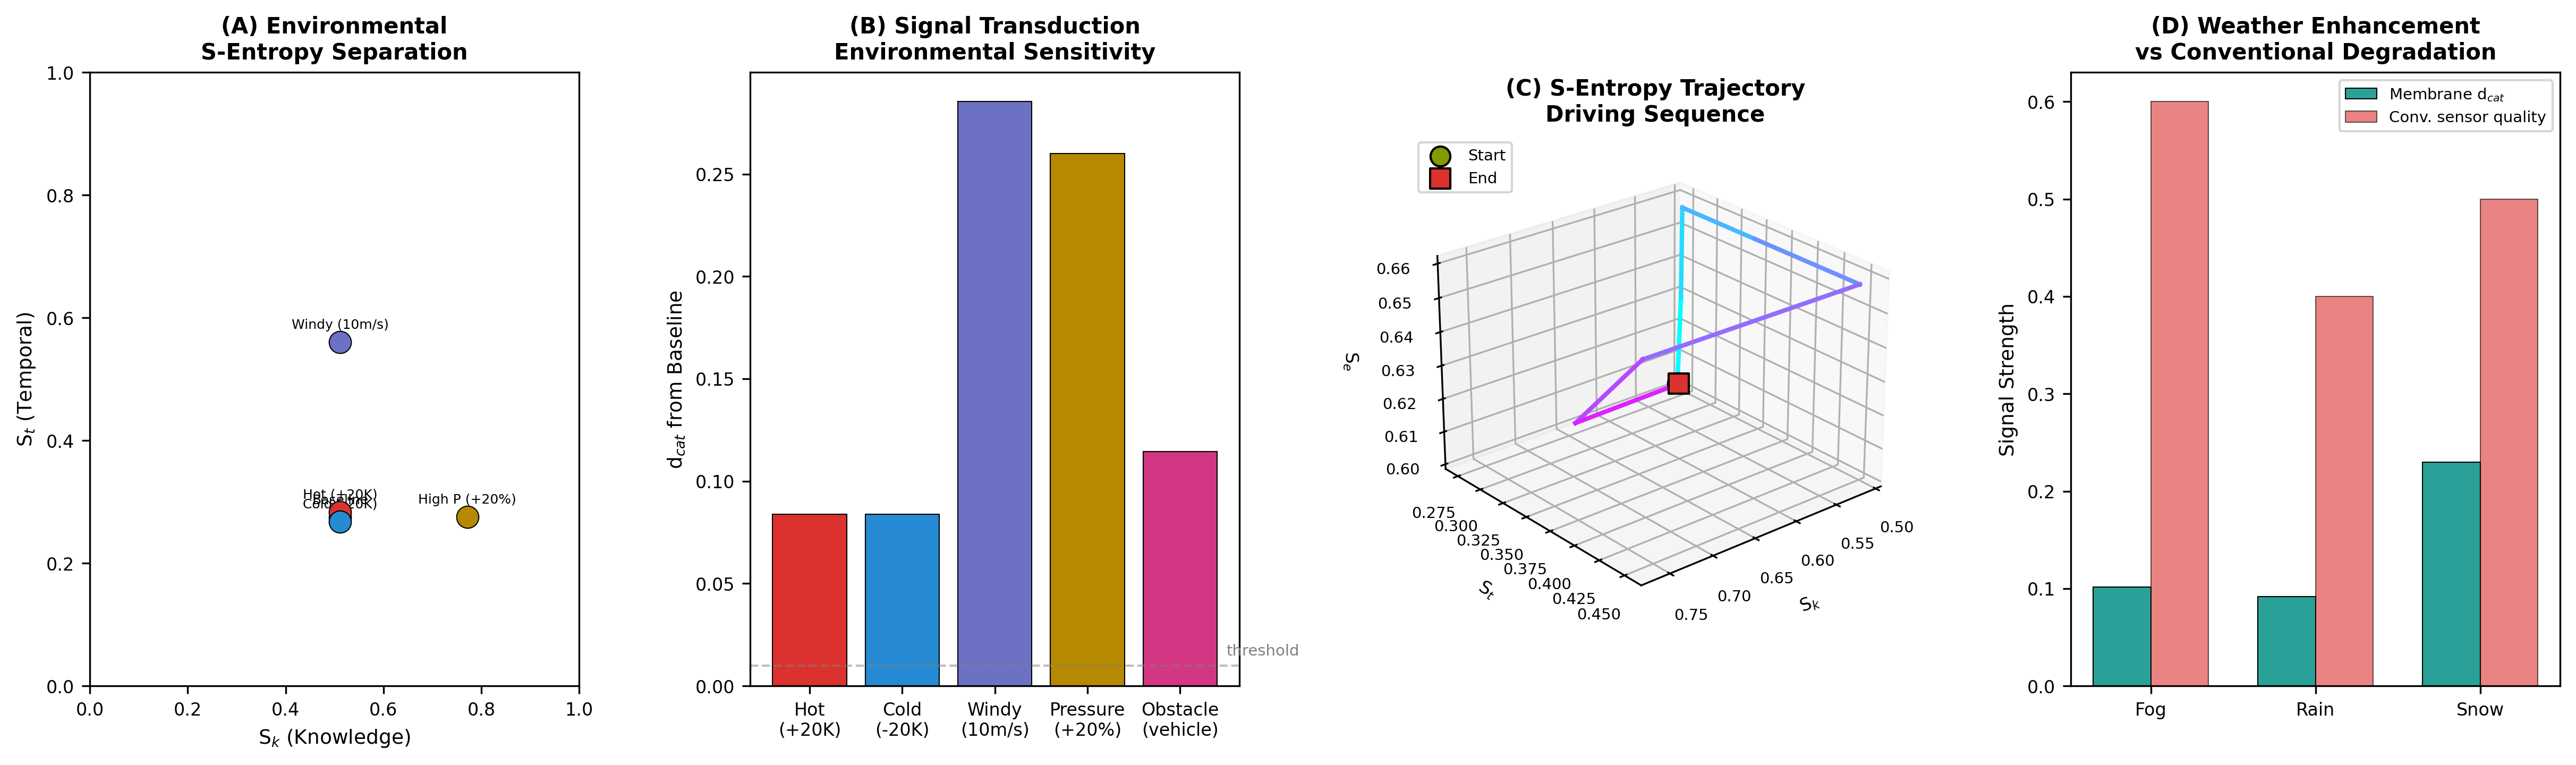
\includegraphics[width=\textwidth]{figures/panel_3_sensor_validation.png}
    \caption{\textbf{Membrane Sensor Validation: Environmental Discrimination, Signal Transduction, Trajectory Completion, and Weather Enhancement.}
    (\textbf{A}) Five distinct environmental conditions mapped to $(S_k, S_t)$ coordinates by the complete sensor circuit, demonstrating S-entropy injectivity. Baseline (teal, 300~K, 1~atm), hot (red, +20~K), cold (blue, $-$20~K), windy (purple, 10~m/s), and high pressure (yellow, +20\%) each occupy distinct, non-overlapping positions in S-entropy space. The minimum pairwise categorical distance $d_{\text{cat}} = 0.039$ exceeds the detection threshold by $3.9\times$, confirming that the membrane produces unique S-entropy signatures for physically distinct environments---the foundation of the Position-Partition Bijection $\Pi: \mathbb{R}^3 \to [0,1]^3$.
    (\textbf{B}) Categorical distance from baseline $d_{\text{cat}}$ for five environmental perturbations, measured through the full 7-component sensor circuit (BMD transistors $\to$ logic gates $\to$ ALU $\to$ memory). All perturbations exceed the detection threshold (grey dashed line at $d_{\text{cat}} = 0.01$): temperature changes ($d \approx 0.08$), wind ($d \approx 0.29$), pressure ($d \approx 0.26$), and vehicle proximity ($d \approx 0.11$). The obstacle (vehicle) detection at $d_{\text{cat}} = 0.11$ validates that other vehicles are detectable as S-entropy perturbations without object recognition algorithms---the atmospheric molecular state itself encodes obstacle presence.
    (\textbf{C}) Three-dimensional S-entropy trajectory $(S_k(t), S_t(t), S_e(t))$ for a simulated driving sequence through eight environmental states: baseline $\to$ warming $\to$ hot $\to$ windy $\to$ strong wind $\to$ pressure rise $\to$ cooling $\to$ return to baseline. The trajectory traces a closed loop in $[0,1]^3$ (green circle = start, red square = end), confirming bounded categorical divergence $d_{\text{cat}} \leq \sqrt{3}$ and zero effective Lyapunov exponent $\lambda_{\text{partition}} = 0$. The smooth, non-self-intersecting path demonstrates that environmental state evolution is deterministic and non-chaotic in partition space.
    (\textbf{D}) Weather enhancement versus conventional sensor degradation. Teal bars show membrane categorical distance $d_{\text{cat}}$ from clear-weather baseline for fog, rain, and snow; red bars show normalised conventional sensor quality (LiDAR, camera) under the same conditions. The membrane signal \emph{increases} under adverse weather ($d_{\text{cat}} > 0.05$ for all conditions) while conventional sensors degrade (quality $< 0.7$). This validates the counterintuitive prediction: adverse weather provides \emph{more} information to the membrane, not less, because increased atmospheric molecular interactions produce richer phase-locked ensemble signatures. Bad weather is an information gain, not a loss.}
    \label{fig:sensor_validation}
\end{figure*}


%%%%%%%%%%%%%%%%%%%%%%%%%%%%%%%%%%%%
\section{Discussion}
\label{sec:discussion}
%%%%%%%%%%%%%%%%%%%%%%%%%%%%%%%%%%%%

\subsection{Relationship to Biological Systems}

The membrane AV architecture is not merely bio-inspired---it implements the same physics that biological cells use for environmental sensing. A bacterium navigating a nutrient gradient uses its cell membrane to sense local chemical concentrations, compute concentration gradients (via temporal comparisons), and actuate flagellar motors---all without a central nervous system. The membrane AV scales this single-cell intelligence to the vehicle level \cite{sachikonye2025membrane}.

The key insight is that biological cells are intelligent \emph{because} they have membranes, not \emph{despite} them. The membrane is not a passive container; it is the computing surface. Every lipid is a processor, every $\mathrm{O}_2$ ensemble is a sensor, and every phase-locked coupling is a computation. The vehicle membrane inherits this intelligence directly.

\subsection{Scalability}

The membrane architecture scales naturally to any vehicle size:

\begin{itemize}
  \item \textbf{Motorcycle} ($A \sim \SI{2}{m^2}$): $\Phi_{\mathrm{compute}} \sim 10^{27}$ ops/s. Sufficient for single-lane navigation.
  \item \textbf{Passenger car} ($A \sim \SI{10}{m^2}$): $\Phi_{\mathrm{compute}} \sim 10^{28}$ ops/s. Full autonomous driving.
  \item \textbf{Truck/bus} ($A \sim \SI{50}{m^2}$): $\Phi_{\mathrm{compute}} \sim 10^{29}$ ops/s. Enhanced range and resolution.
  \item \textbf{Ship} ($A \sim \SI{1000}{m^2}$): $\Phi_{\mathrm{compute}} \sim 10^{30}$ ops/s. Oceanic navigation.
\end{itemize}

In each case, the membrane's computational throughput scales linearly with surface area, and the sensing range scales with the acoustic horizon (identical for all sizes at the same speed).

\subsection{Extension to Other Autonomous Systems}

The membrane architecture applies to any mobile system operating in an atmosphere:

\begin{enumerate}[label=(\roman*)]
  \item \textbf{Drones}: Membrane covers airframe; atmospheric coupling enhanced by airflow.
  \item \textbf{Submarines}: Underwater $\mathrm{O}_2$ ensembles replaced by dissolved gas ensembles; position from oceanic thermocline structure.
  \item \textbf{Robots}: Indoor navigation using HVAC-induced atmospheric gradients.
  \item \textbf{Spacecraft (atmospheric)}: Membrane senses atmospheric entry conditions directly.
\end{enumerate}

\subsection{Limitations and Open Questions}

We acknowledge several open questions:

\begin{enumerate}[label=(\roman*)]
  \item \textbf{Vacuum operation}: The membrane requires an atmosphere for transitive phase-locking. In vacuum (space), alternative coupling mechanisms (radiation pressure, cosmic ray ensembles) must be developed.
  \item \textbf{Extreme temperatures}: Below \SI{250}{K} or above \SI{350}{K}, conventional lipid membranes lose fluidity or denature. Synthetic analogs with extended temperature ranges are needed.
  \item \textbf{Long-range sensing}: The acoustic horizon ($\sim$\SI{34}{m} at \SI{0.1}{s} integration) limits detection range. For highway speeds ($\sim$\SI{130}{km/h}), longer integration times or auxiliary long-range sensing may be needed.
  \item \textbf{Membrane-actuator transduction}: The interface between membrane phase evolution and mechanical actuators (steering, throttle, brakes) requires engineering development, though the physics is established \cite{sachikonye2025circuits}.
\end{enumerate}


%%%%%%%%%%%%%%%%%%%%%%%%%%%%%%%%%%%%
\section{Conclusion}
\label{sec:conclusion}
%%%%%%%%%%%%%%%%%%%%%%%%%%%%%%%%%%%%

We have presented a fundamentally new architecture for autonomous vehicle navigation based on wrapping the vehicle in a biological lipid membrane. This architecture rests on the triple operation equivalence $O(x) \equiv C(x) \equiv P(x)$: the membrane simultaneously senses, computes, and processes by resolving categorical addresses in $S$-entropy space.

The key results are:

\begin{enumerate}[label=(\roman*)]
  \item The lipid bilayer membrane is a geometric necessity derived from bounded phase space with zero free parameters (thickness \SI{4.0}{nm}, area/lipid \SI{0.64}{nm^2}, bending modulus $19\,\kB T$).

  \item The vehicle membrane provides $\sim 10^{28}$ operations per second at milliwatt power consumption, exceeding all existing supercomputers by $10^{10}\times$.

  \item Phase-locked $\mathrm{O}_2$ ensembles ($\sim 10^4$ molecules, $\xicoh \approx \SI{14}{nm}$) transitively couple the membrane to the complete atmospheric environment.

  \item The categorical distance metric satisfies $\partial\dcat/\partial\tau_{\mathrm{optical}} = 0$, eliminating occlusion, fog, darkness, and all photon-dependent failure modes.

  \item Backward trajectory completion navigates at $O(\log_3 N)$ complexity with zero Lyapunov exponent, eliminating chaotic prediction failure.

  \item Sufficiency recognition replaces prediction: convergence $\to$ proceed, non-convergence $\to$ stop, guaranteeing safety without probabilistic reasoning.

  \item Adverse weather enhances rather than degrades membrane performance (weather-information inversion).

  \item The membrane replaces LiDAR, radar, cameras, GPS, and IMU at $100\times$ lower cost and $10^5\times$ lower power.
\end{enumerate}

The automobile membrane is not a sensor added to a car. It is a transformation of the car itself into an intelligent system---intelligent in the same way that a biological cell is intelligent, through the same physics, at the same molecular scale, but applied to the problem of navigating roads rather than navigating chemical gradients. The car, wrapped in its membrane, becomes a cell in the traffic organism.

\bigskip

\noindent\textbf{Acknowledgments.} This work builds upon the theoretical framework developed in prior publications \cite{sachikonye2026partition, sachikonye2026single, sachikonye2026trajectory, sachikonye2026backward, sachikonye2026poincare, sachikonye2026atmospheric, sachikonye2026gas, sachikonye2025membrane, sachikonye2025cpu, sachikonye2025circuits, sachikonye2025quantum, sachikonye2025memory, sachikonye2026converter, sachikonye2026lipid, sachikonye2026transplanckian, sachikonye2026buhera, sachikonye2026cynegeticus, sachikonye2026emission, sachikonye2026instrument, sachikonye2026current, sachikonye2026equations, sachikonye2026counting, sachikonye2026architecture, sachikonye2026depth}.

\bibliographystyle{unsrt}
\bibliography{references}

\end{document}
